\chapter{嗅觉和味觉:化学感觉} \label{chap:chap29}

通过嗅觉和味觉,我们能够感知到外部世界中数量惊人、种类繁多的化学物质。
这些化学感官告诉我们食物的可用性及其潜在的快乐或危险。
嗅觉和味觉也会引发消化和利用食物所需的生理变化。
在许多动物中,嗅觉系统还通过检测引发先天行为或生理反应的信息素发挥重要的社会功能。


尽管与许多其他动物相比,人类的辨别能力有些有限,但气味化学家估计人类的嗅觉系统可能能够检测 1 万多种不同的挥发性化学物质。
经过严格训练以辨别气味的调香师可以区分多达 5 千种不同类型的气味,品酒师可以根据风味和香气的组合辨别 1 百多种不同的味道成分。


在本章中,我们将考虑气味和味觉刺激是如何被检测到的,以及它们是如何编码成神经信号模式传输到大脑的。
近年来,人们对各种动物物种化学感应的潜在机制有了很多了解。
化学感应的某些特征在进化过程中得以保留,而其他特征则是个别物种的特殊适应。



\section{一大群嗅觉受体启动嗅觉}

气味物质——被感知为气味的挥发性化学物质——被鼻子中的嗅觉感觉神经元检测到。
感觉神经元嵌入鼻腔一部分的特殊\textit{嗅上皮}细胞中,人类面积约为 5 平方厘米(图~\ref{fig:29_1}),并散布着神经胶质样支持细胞(图~\ref{fig:29_2})。
它们的寿命相对较短,寿命只有 30 到 60 天,由上皮中的一层基底干细胞不断更新。


\begin{figure}[htbp]
	\centering
	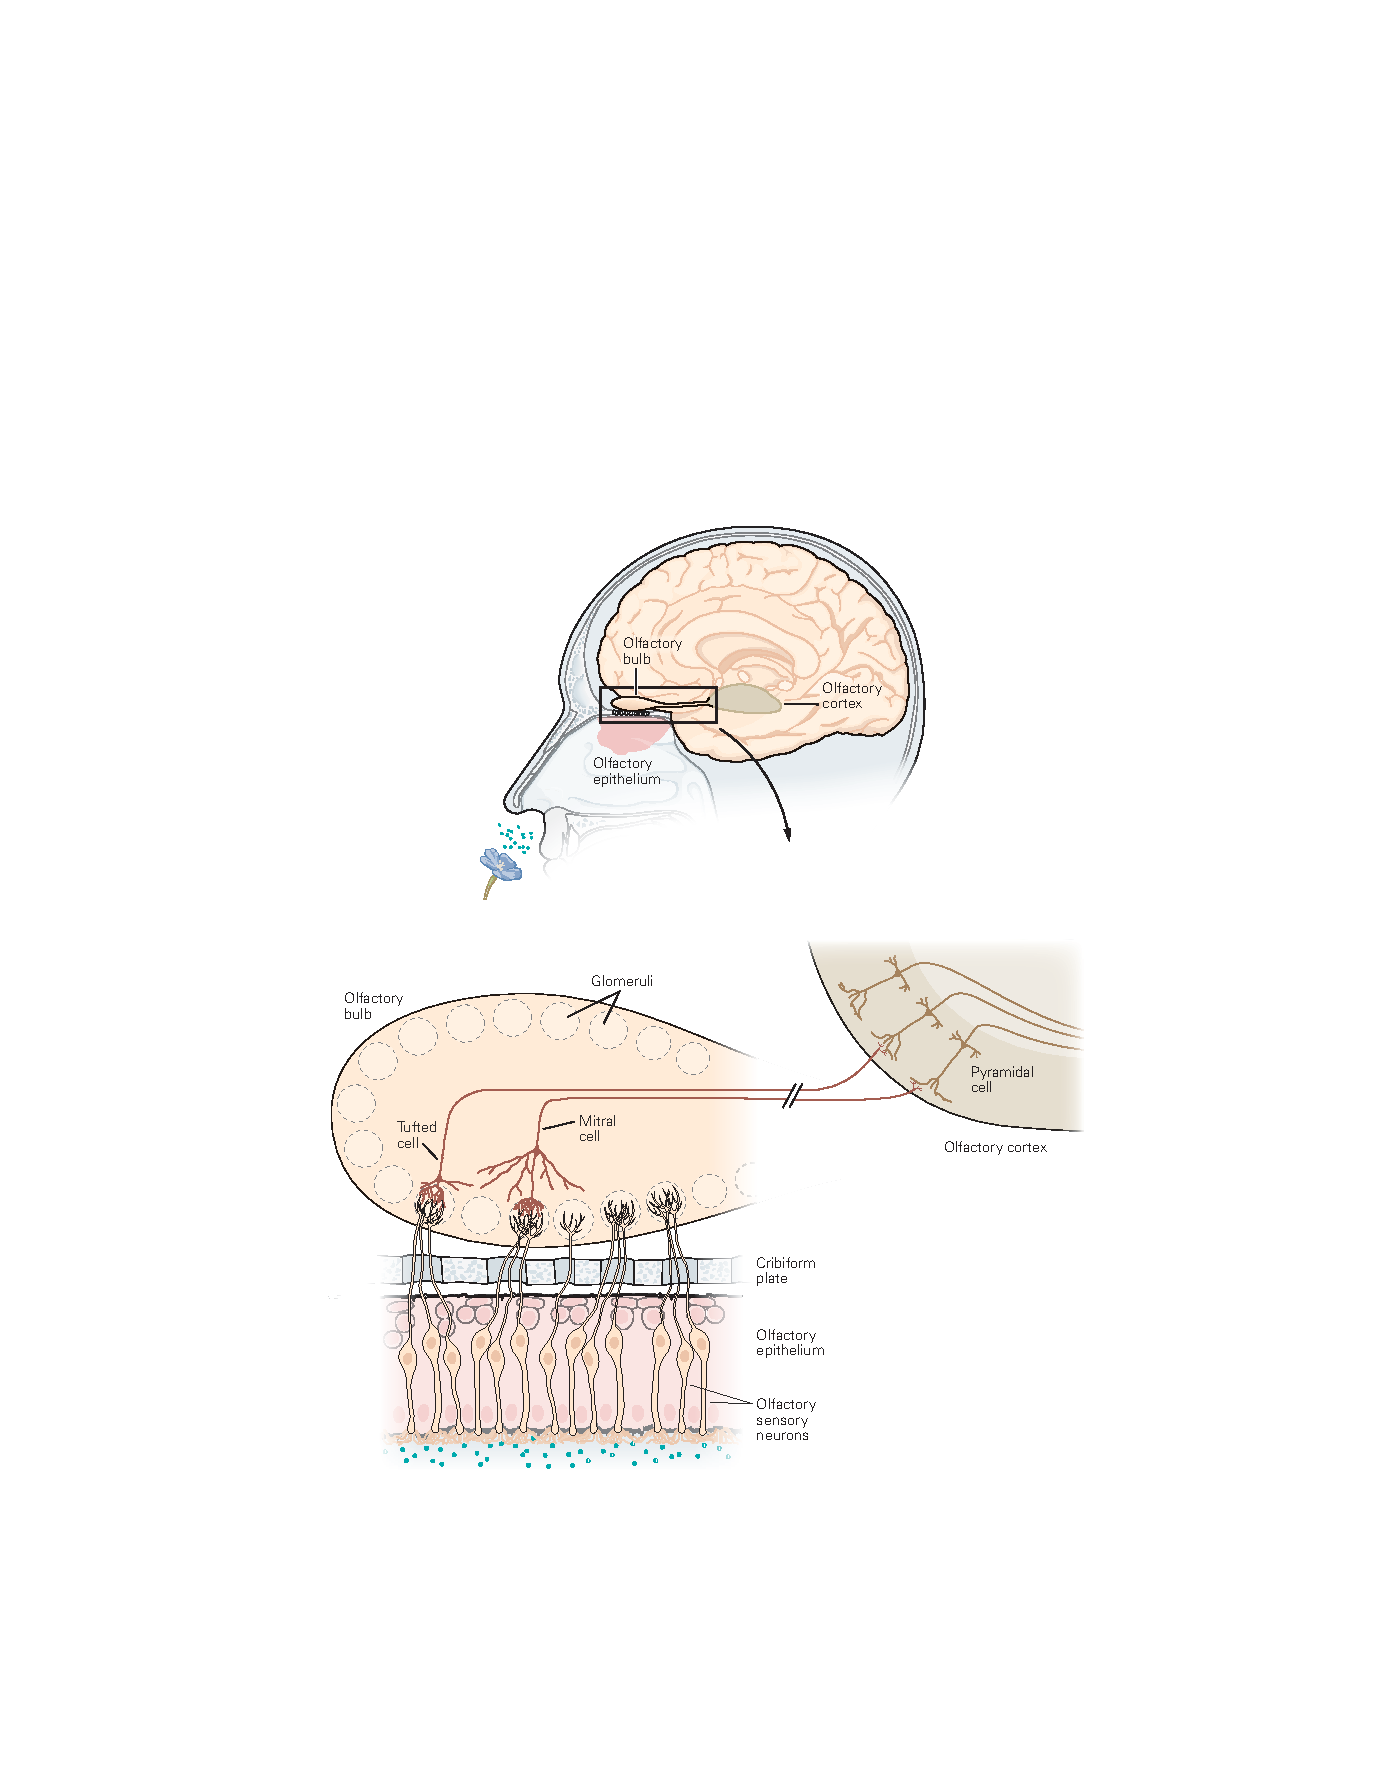
\includegraphics[width=0.7\linewidth]{chap29/fig_29_1}
	\caption{嗅觉系统。
	\textit{嗅上皮}细胞中的\textit{嗅觉感觉神经元}检测到气味,\textit{嗅上皮}细胞排列在鼻腔的一部分。
	这些神经元的轴突投射到嗅球,在那里它们终止于\textit{僧帽细胞}的树突和肾小球内的簇状细胞中继神经元。
	反过来,中继神经元的轴突投射到\textit{嗅觉皮层},在那里它们终止于锥体神经元的树突,而锥体神经元的轴突投射到其他大脑区域。}
	\label{fig:29_1}
\end{figure}


\textit{嗅觉感觉神经元}是双极神经细胞。
单个树突从顶端延伸到上皮表面,在那里它产生许多细纤毛,伸入覆盖鼻腔的粘液中(图~\ref{fig:29_2})。
纤毛含有气味受体以及放大来自受体的感觉信号并将其转化为神经元轴突中的电信号所需的转导机制,轴突从神经元的基底极投射到大脑。
嗅觉感觉神经元的轴突穿过筛板(鼻腔上方颅骨中的穿孔区域),然后终止于嗅球(见图~\ref{fig:29_1})。


\begin{figure}[htbp]
	\centering
	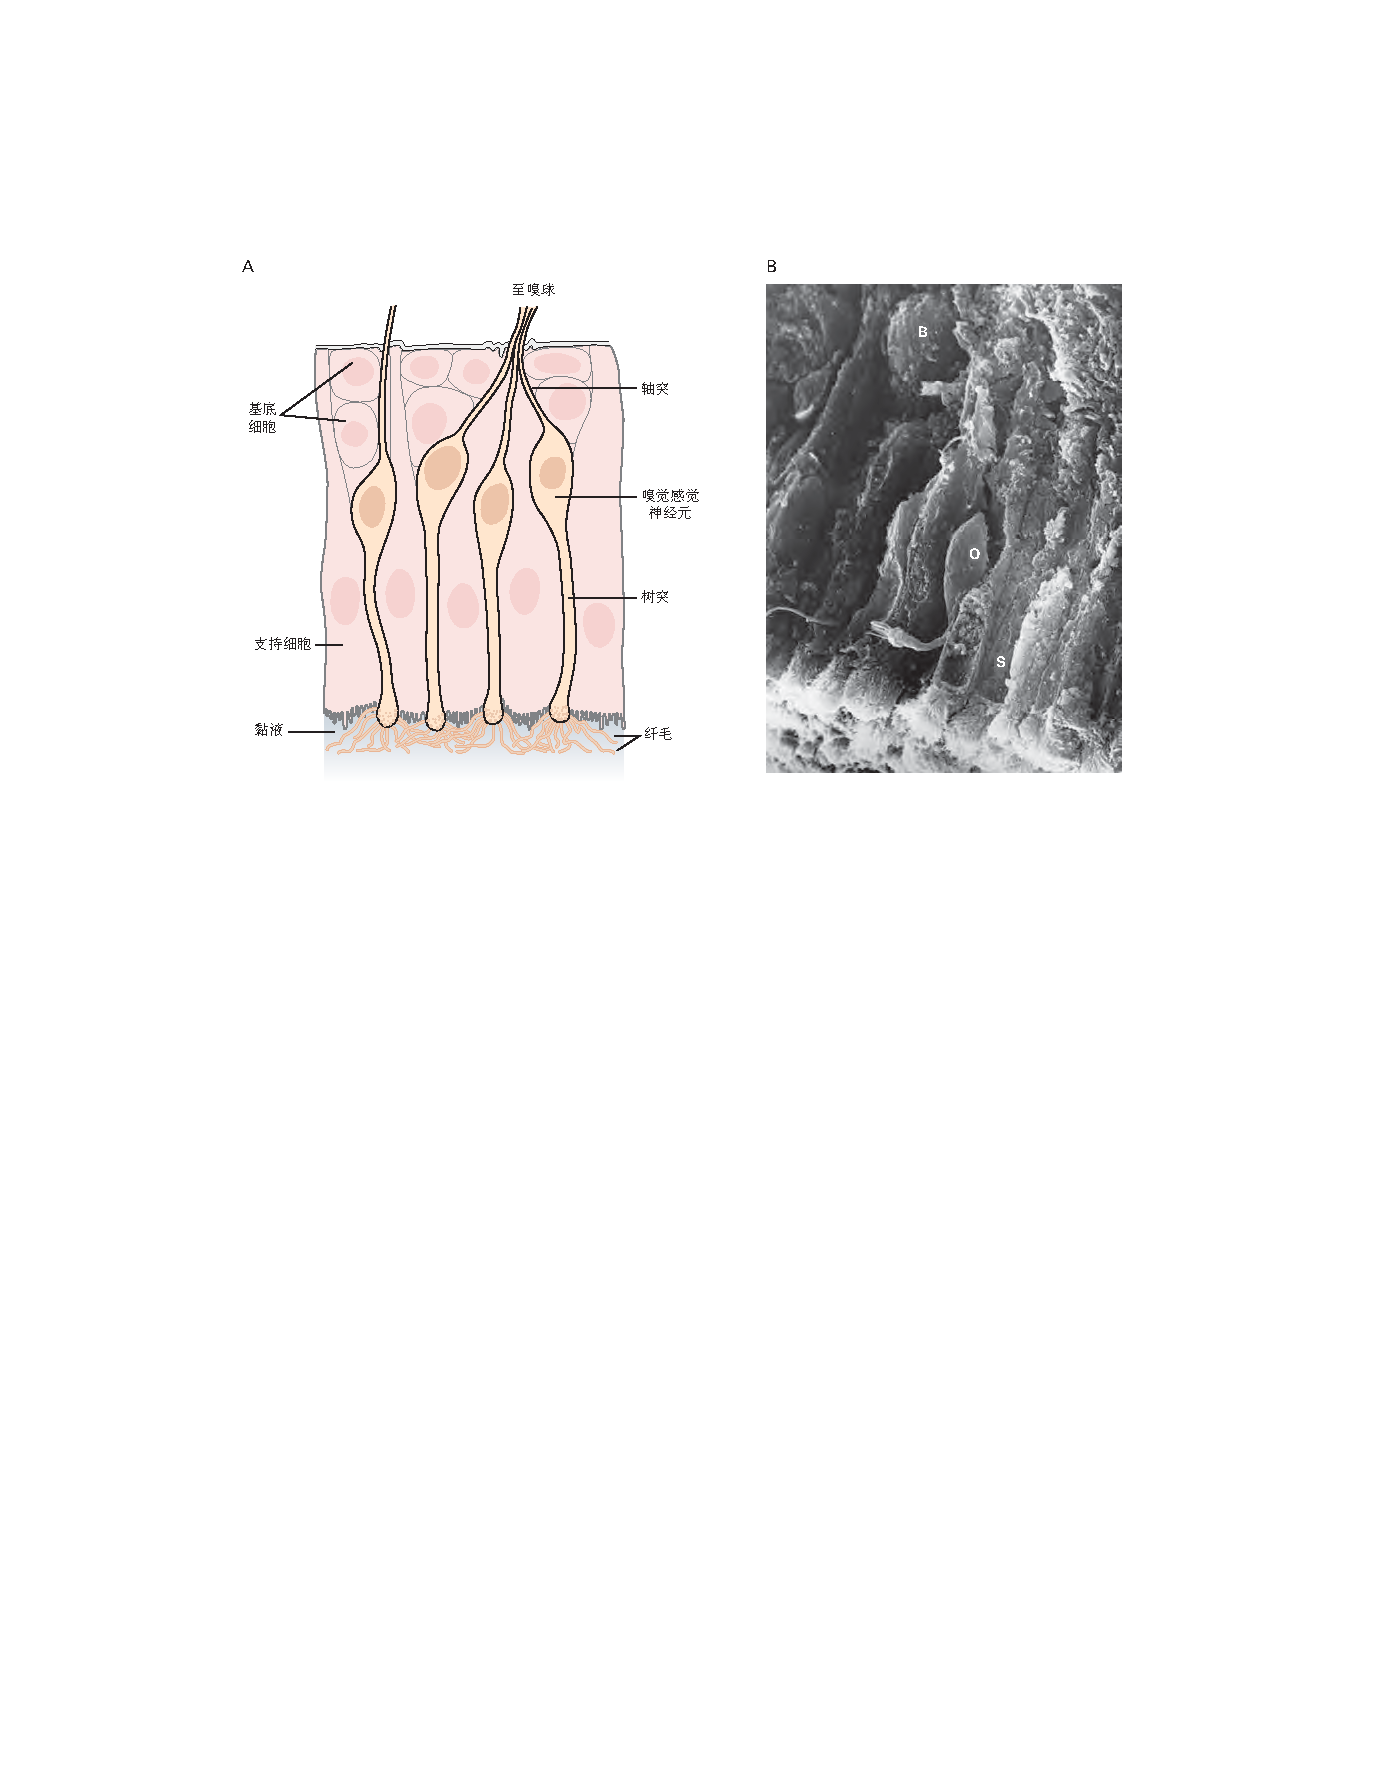
\includegraphics[width=0.8\linewidth]{chap29/fig_29_2}
	\caption{\textit{嗅上皮}。
	\textbf{A.} \textit{嗅上皮}细胞包含散布着支持细胞的感觉神经元以及干细胞基底层。
	单个树突从每个神经元的顶端延伸;
	感觉纤毛从树突末端发芽进入鼻腔内壁的粘液中。
	轴突从每个神经元的基端延伸到嗅球。
	\textbf{B.} \textit{嗅上皮}的扫描电子显微照片显示上皮表面有密集的感觉纤毛垫。
	\textit{支持细胞} (S) 是柱状细胞,延伸到上皮细胞的整个深度并具有顶端微绒毛。
	散布在支持细胞中的是一个带有树突和纤毛的\textit{嗅觉感觉神经元} (O),以及一个基底干细胞 (B)。}
	\label{fig:29_2}
\end{figure}



\subsection{哺乳动物共享一大类气味受体}

气味受体是由多基因家族编码的蛋白质,该家族在进化上是保守的,存在于所有脊椎动物物种中。
人类有大约 350 种不同的气味受体,而小鼠大约有 1 千种。 
尽管气味受体属于 G 蛋白偶联受体超家族,但它们共享其他超家族成员中未见的序列基序。
值得注意的是,气味受体的氨基酸序列差异很大(图~\ref{fig:29_3}A)。


\begin{figure}[htbp]
	\centering
	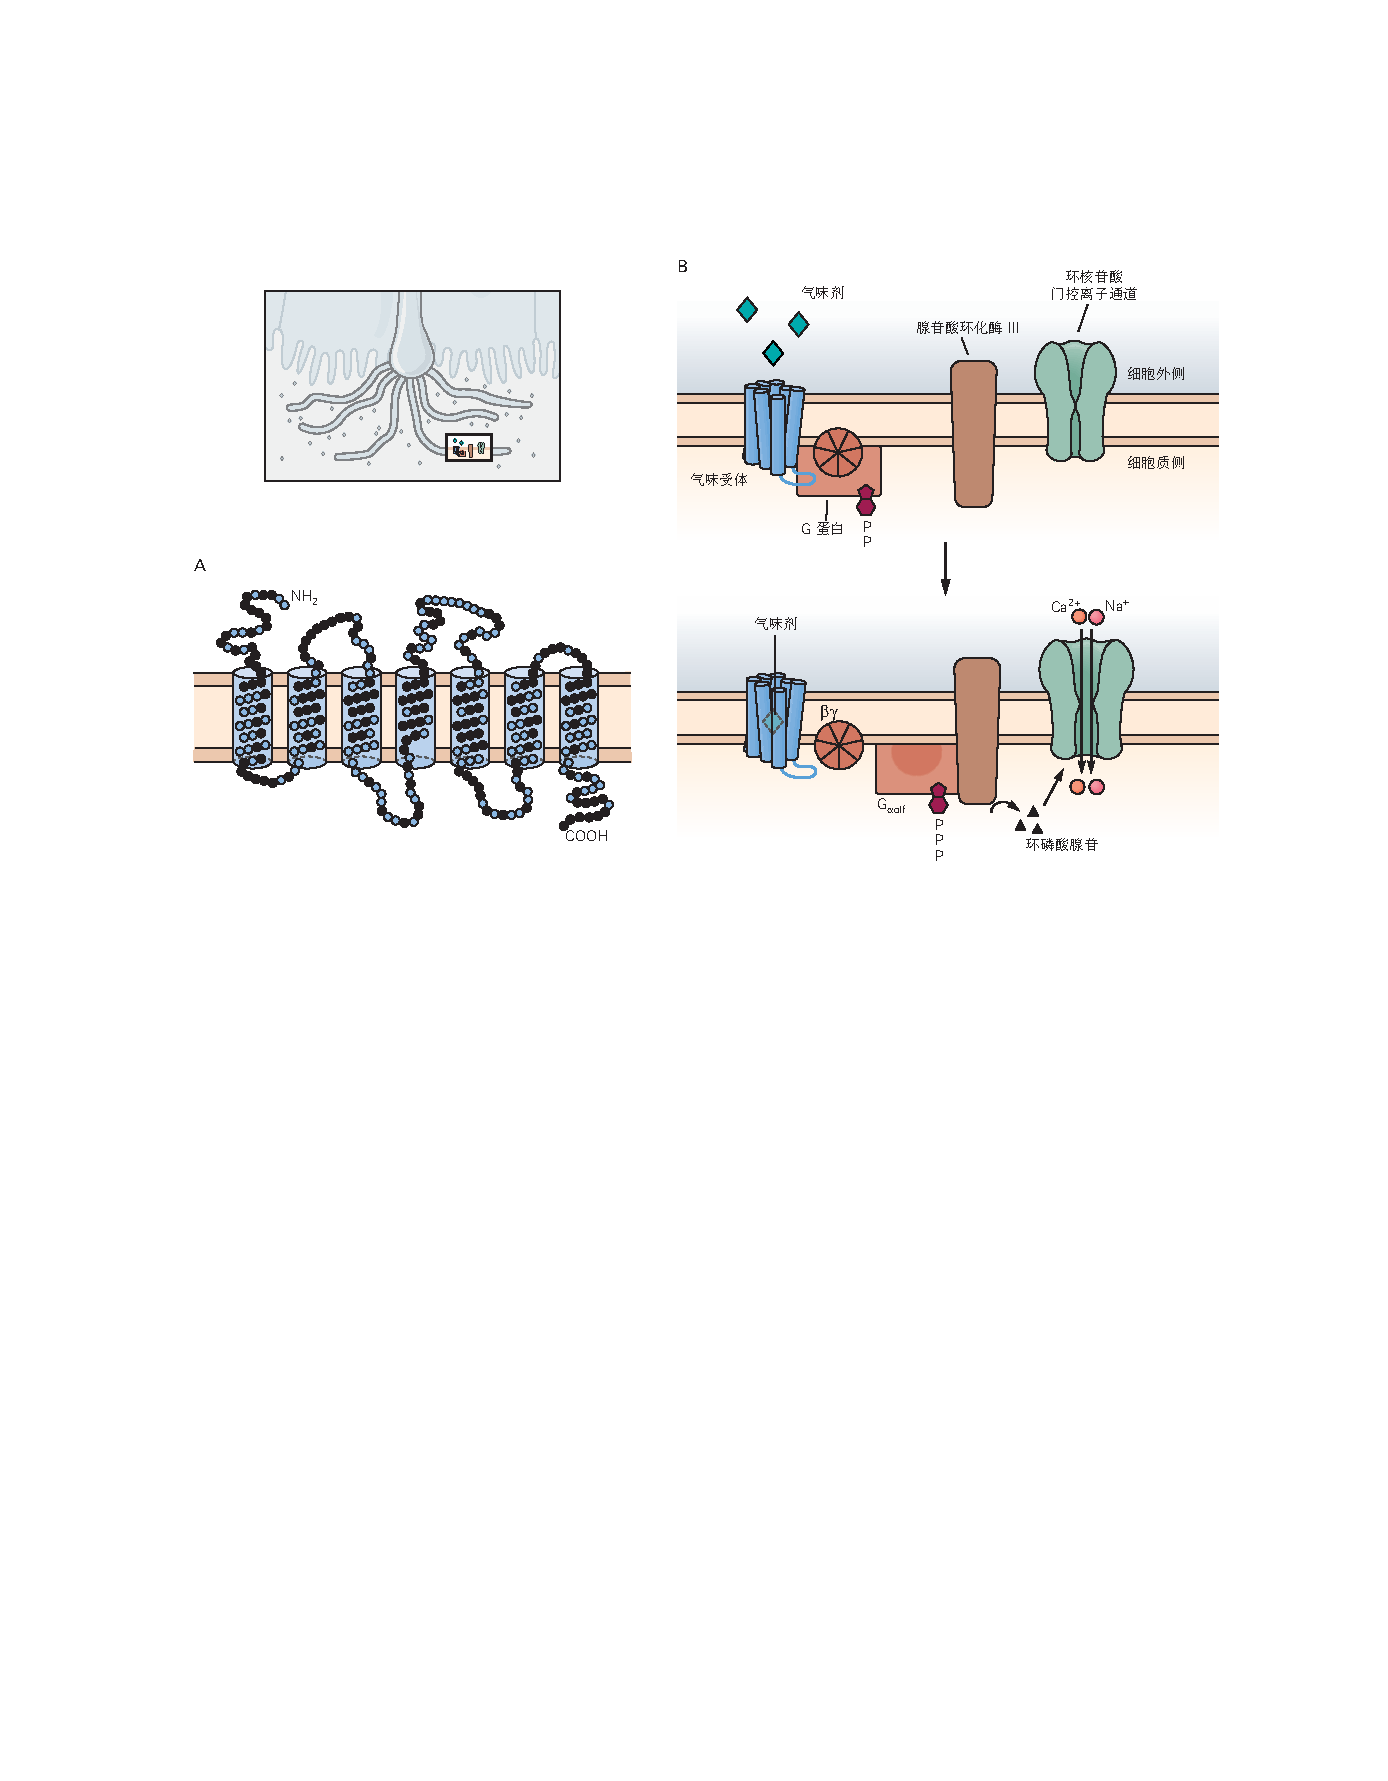
\includegraphics[width=0.95\linewidth]{chap29/fig_29_3}
	\caption{气味受体。
		\textbf{A.} 气味受体具有 G 蛋白偶联受体特有的七个跨膜结构域。
		它们彼此相关但氨基酸序列不同(变异性最高的位置在这里显示为黑球)。
		\textbf{B.} 气味剂的结合导致气味剂受体与异源三聚体 G 蛋白的 $ \alpha $ 亚基 Gαolf 相互作用。
		这导致\textit{三磷酸鸟苷}偶联的 G$_\alpha olf $ 的释放,它刺激腺苷酸环化酶 III,导致\textit{环磷酸腺苷}增加。
		升高的\textit{环磷酸腺苷}反过来诱导环核苷酸门控阳离子通道的打开,导致阳离子流入和睫状膜中膜电位的变化。}
	\label{fig:29_3}
\end{figure}


与其他 G 蛋白偶联受体一样,气味受体有七个可能用作跨膜结构域的疏水区域(图~\ref{fig:29_3}A)。
对其他 G 蛋白偶联受体(例如 $\beta$-肾上腺素能受体)的详细研究表明,气味结合发生在由跨膜结构域组合形成的跨膜区域的口袋中。
气味受体的氨基酸序列在几个跨膜结构域中尤其可变,这为气味结合口袋的可变性提供了可能的基础,这可以解释不同受体识别结构不同的配体的能力。


第二个较小的化学感应受体家族也在\textit{嗅上皮}细胞中表达。
这些受体称为\textit{微量胺相关受体},是 G 蛋白偶联的,但它们的蛋白质序列与气味受体的蛋白质序列无关。 
它们由存在于人类和小鼠以及鱼类中的一小部分基因编码。
对具有 14 种不同嗅觉\textit{微量胺相关受体}的小鼠进行的研究表明,\textit{微量胺相关受体}可识别挥发性胺,其中一种以高浓度存在于雄性小鼠的尿液中,另一种则存在于某些捕食者的尿液中。
这个小受体家族可能具有不同于气味受体家族的功能,可能与检测动物线索有关。
另一个由 12 种受体组成的家族,称为 MS4Rs,也在小鼠中发现,它可能参与信息素和某些食物气味的检测。


气味剂与其受体的结合会引发一系列细胞内信号事件,从而使嗅觉感觉神经元去极化(图~\ref{fig:29_3}B)。
去极化被动地扩散到细胞体,然后是轴突,在那里产生的动作电位被主动传导到嗅球。


人类和其他动物会迅速适应气味,例如对持续存在的难闻气味的检测减弱。
当暂时去除气味时,感知气味的能力会迅速恢复。
对气味的适应部分是由嗅觉纤毛中环核苷酸门控离子通道的调节引起的,但敏感性迅速恢复的机制尚不清楚。



\subsection{不同的受体组合编码不同的气味}

为了在感知上加以区分,不同的气味必须引起不同的信号从鼻子传递到大脑。
这是通过两种方式实现的。
首先,每个嗅觉感觉神经元只表达一个气味受体基因,因此是一种受体。 
其次,每个受体识别多种气味,相反,每种气味被多个不同的受体检测到(图~\ref{fig:29_4})。 
然而,重要的是,每种气味都会被独特的受体组合检测到,并因此被编码,从而导致一种独特的信号模式被传输到大脑。


\begin{figure}[htbp]
	\centering
	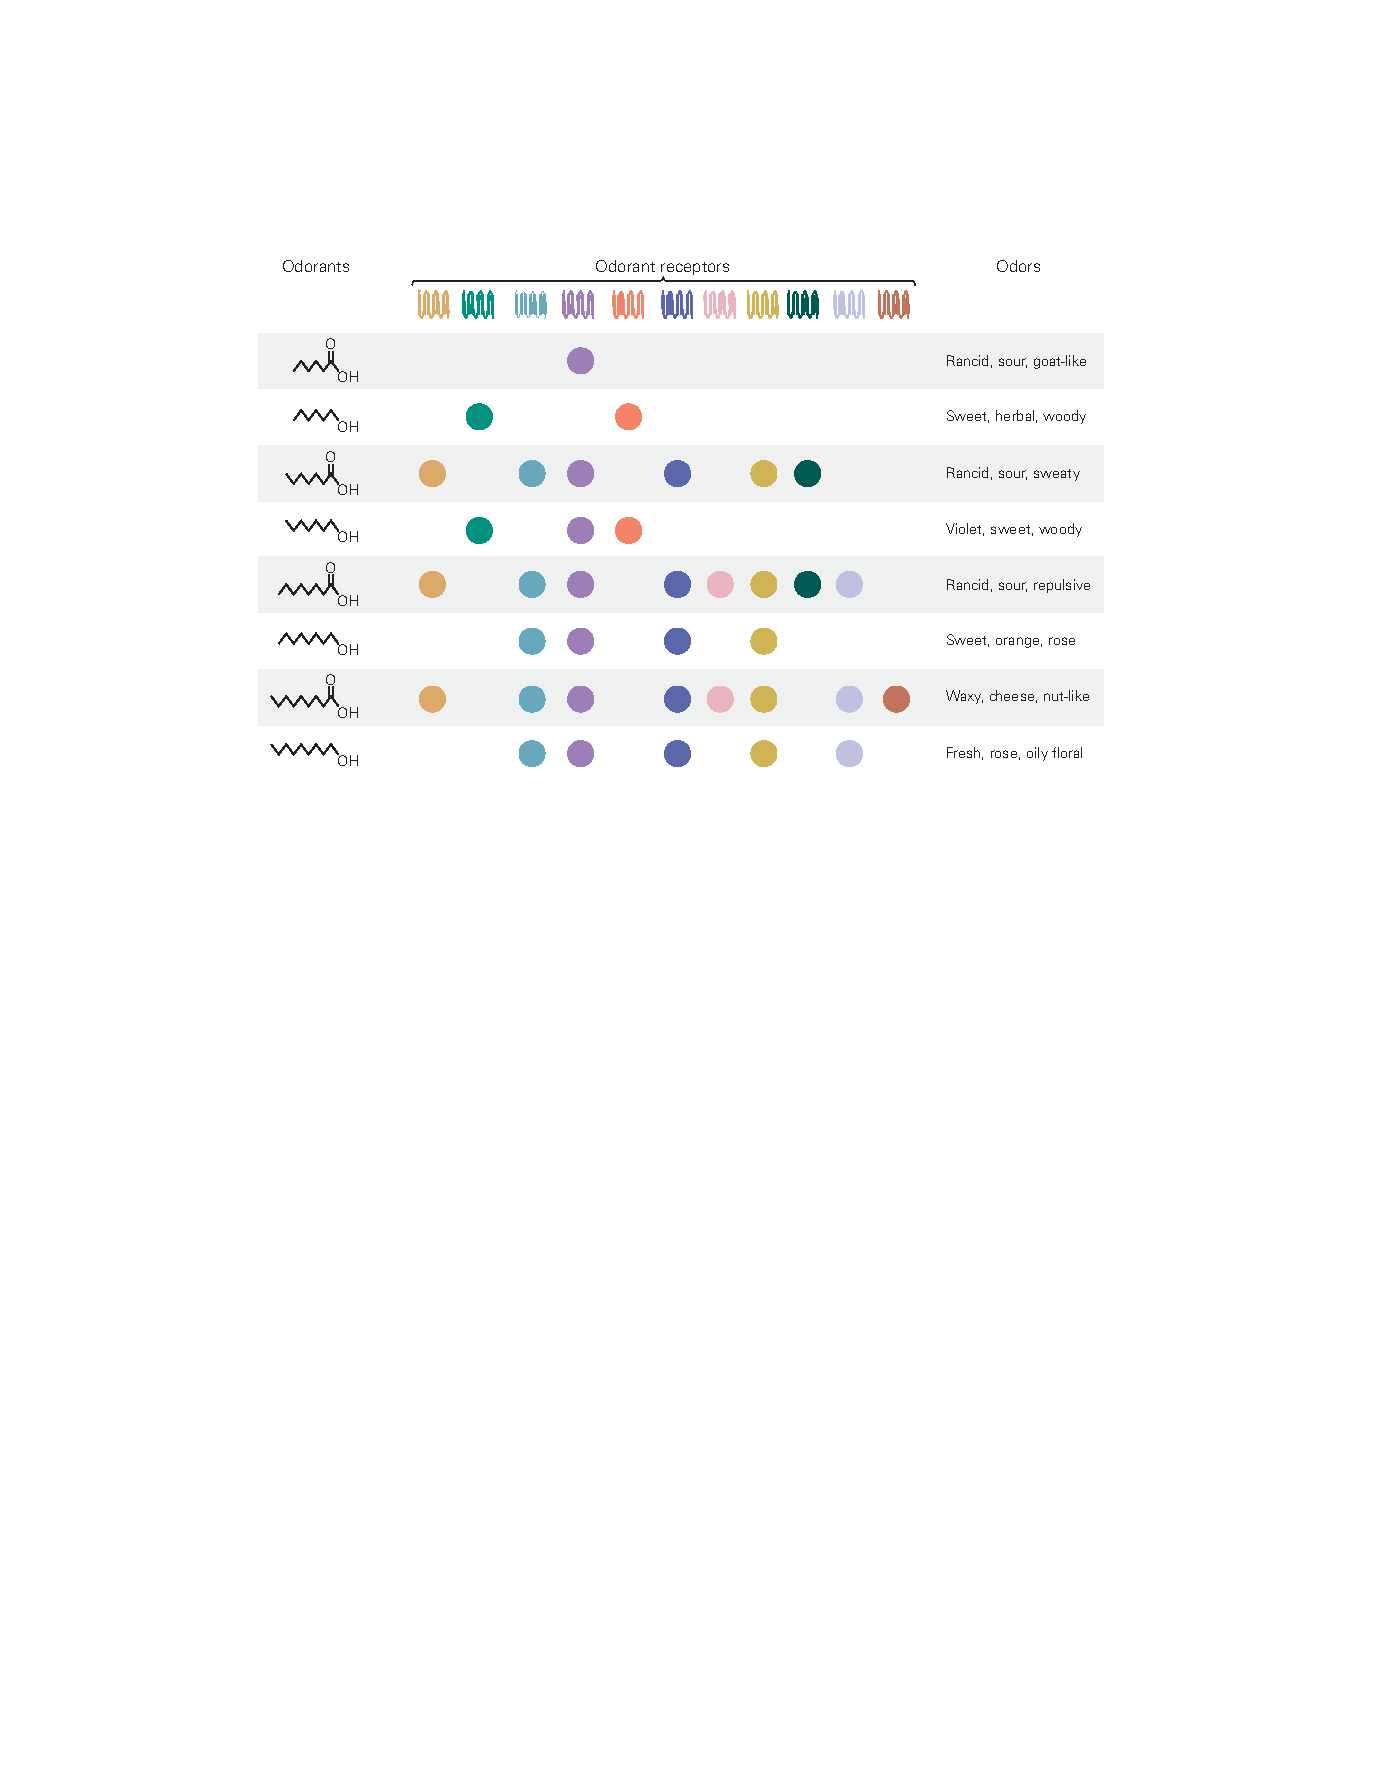
\includegraphics[width=0.8\linewidth]{chap29/fig_29_4}
	\caption{每种气味都被独特的受体组合所识别。
		单一的气味受体可以识别多种气味,但不同的气味会被不同的受体组合检测到,并因此被编码。
		这种组合编码解释了哺乳动物如何将具有相似化学结构的气味剂区分为具有不同的气味。
		图中的数据是通过用不同的气味测试小鼠嗅觉感觉神经元,然后确定每个反应神经元表达的气味受体基因得到的。
		右侧显示的人类对这些气味的感知质量说明了高度相关的气味如何具有不同的气味\cite{malnic1999combinatorial}。}
	\label{fig:29_4}
\end{figure}


气味的组合编码极大地扩展了嗅觉系统的辨别能力。
如果每种气味只被三种不同的受体检测到,那么这种策略理论上可以产生数百万种不同的组合受体编码——以及从鼻子发送到大脑的数量相当多的不同信号模式。
有趣的是,即使结构几乎相同的气味也会被不同的受体组合识别(图~\ref{fig:29_4})。
高度相关的气味剂具有不同的组合受体编码这一事实解释了为什么气味剂化学结构的轻微变化可以改变其感知的气味。
在某些情况下,结果是戏剧性的,例如,将化学物质的感觉从玫瑰色变为酸味。


有气味物质浓度的变化也会改变感知到的气味。
例如,低浓度的硫萜品醇闻起来像热带水果,而较高浓度闻起来像葡萄柚,甚至更高浓度闻起来有腐臭味。
随着气味浓度的增加,对气味具有较低亲和力的其他受体被募集到反应中,从而改变组合受体编码,从而解释气味浓度对感知的影响。



\section{嗅觉信息沿着通往大脑的通路转化}

\subsection{气味由分散在鼻子中的神经元编码}

来自大量不同气味受体的信号如何在神经系统中组织起来以产生不同的气味感知呢?
这个问题已经在啮齿动物中进行了研究。
对老鼠的研究表明,嗅觉信息在从\textit{嗅上皮}细胞到\textit{嗅球}再到\textit{嗅觉皮层}的过程中经历了一系列的转变。


\textit{嗅上皮}细胞具有一系列表达不同嗅觉受体的空间区域。
每种受体类型在限制在一个大约 5 千个神经元的区域中表达(图~\ref{fig:29_5})。
(回想一下,每个神经元只表达一个气味受体基因。)
具有相同受体的神经元随机散布在一个区域内,因此具有不同受体的神经元散布在一起。
所有区域都包含多种受体,并且特定的气味可能被不同区域的受体识别。
因此,尽管气味受体大致组织成空间区域,但气味受体家族提供的信息高度分布在上皮细胞中。


\begin{figure}[htbp]
	\centering
	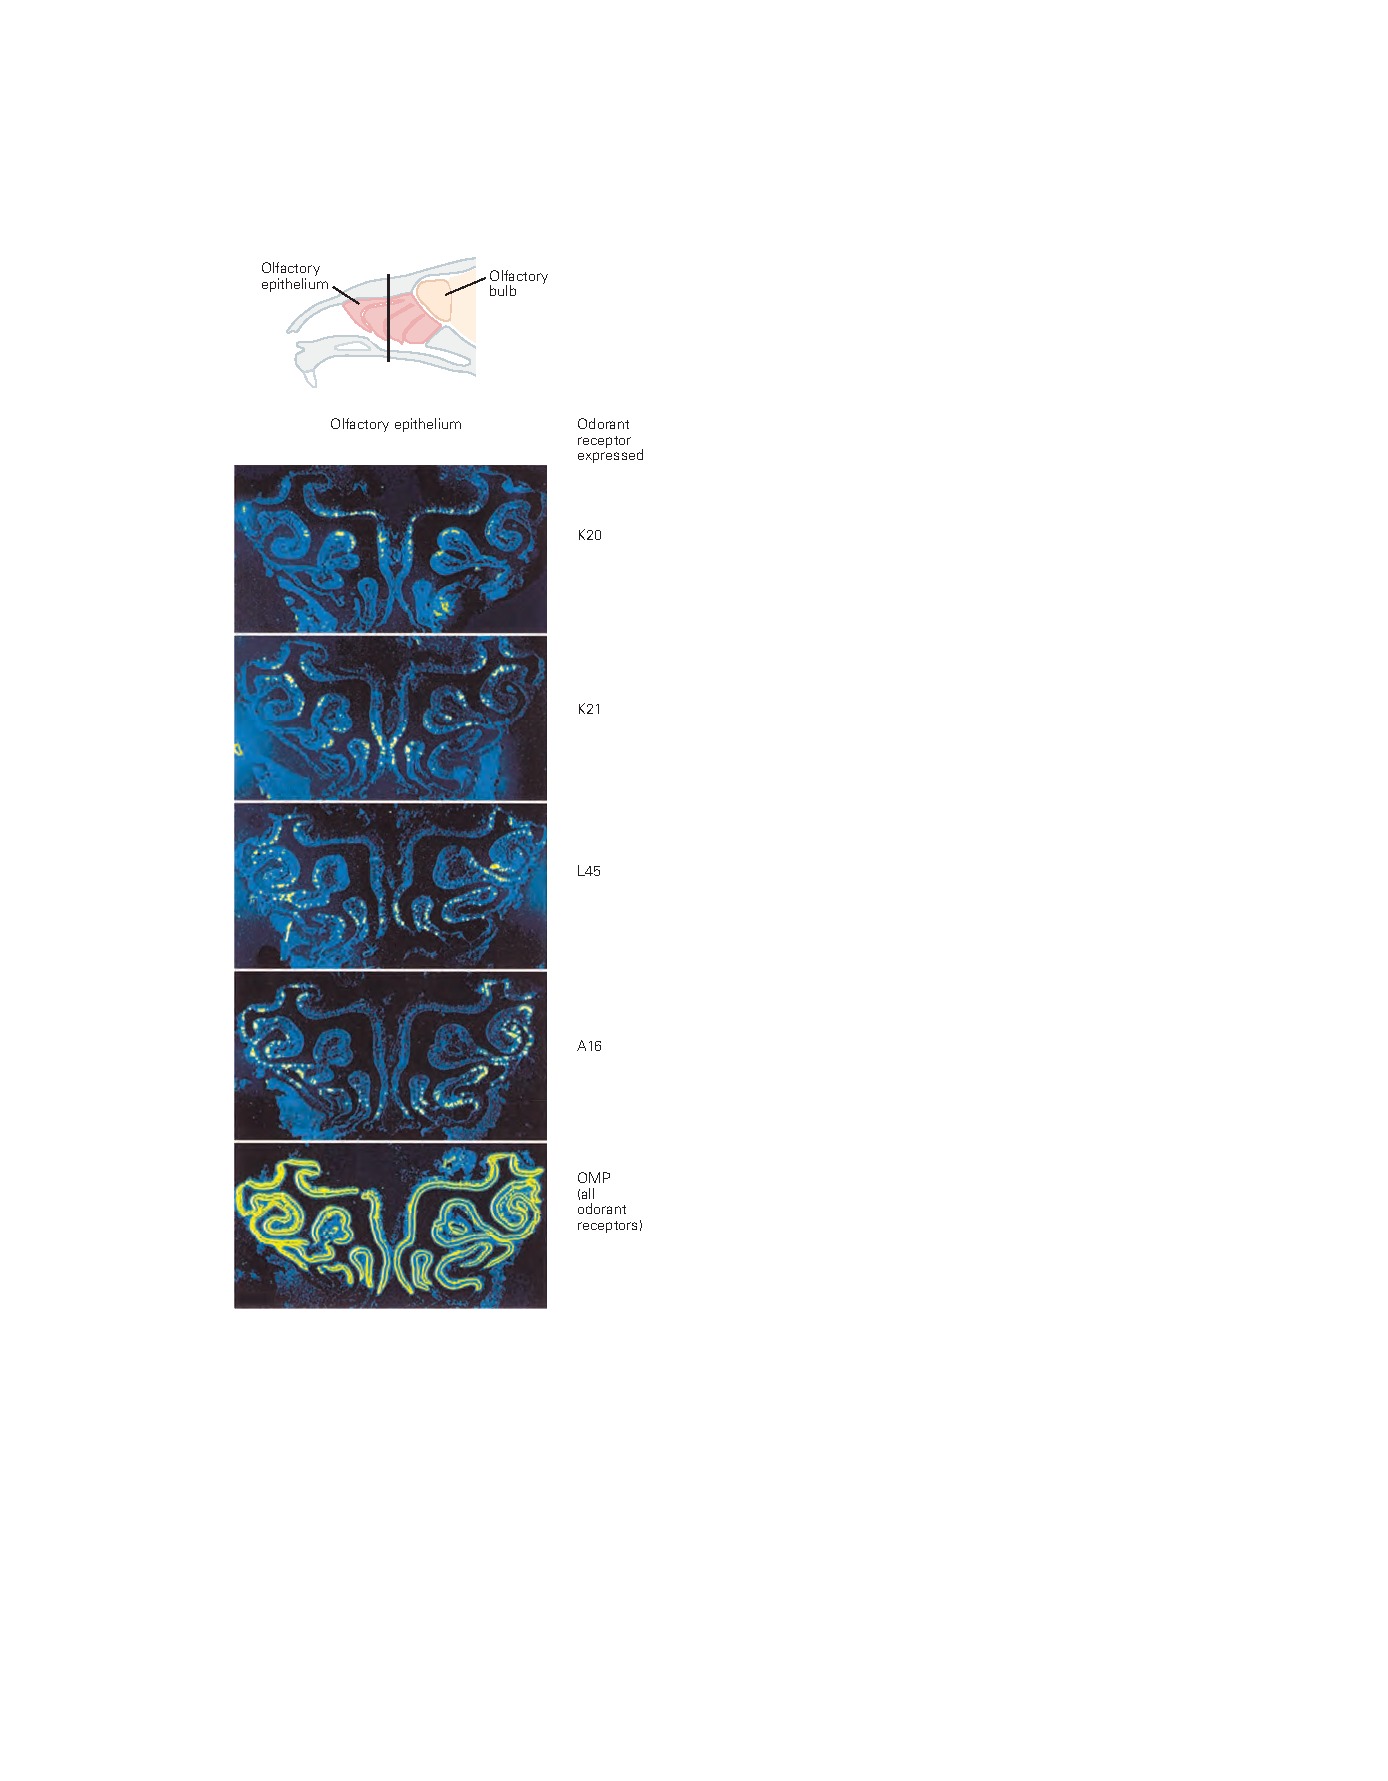
\includegraphics[width=0.5\linewidth]{chap29/fig_29_5}
	\caption{\textit{嗅上皮}中感觉输入的组织。
		\textit{嗅上皮}具有不同的空间区域,可以表达不同的气味受体基因组。
		每个感觉神经元仅表达一个受体基因,因此是一种类型的受体。
		具有相同受体的神经元被限制在一个区域内,但随机散布在该区域内,因此具有不同受体的神经元散布在一起。
		显微照片显示了通过小鼠鼻子的切片中四种不同受体探针标记的神经元分布。
		\textit{嗅觉标记蛋白}探针标记所有表达气味受体的神经元\cite{ressler1993zonal}。
		图~\ref{fig:29_6}~嗅球中间神经元。
		除了兴奋性\textit{僧帽细胞}和簇状中继神经元外,嗅球还含有抑制性中间神经元。
		在每个肾小球内,\textit{$\gamma$-氨基丁酸}能球周细胞的树突接收来自嗅觉感觉神经元的兴奋性输入,并与\textit{僧帽细胞}和簇状中继神经元的初级树突形成相互突触,表明可能在信号修饰中发挥作用。
		嗅球深处的\textit{$\gamma$-氨基丁酸能}颗粒细胞的树突与中继神经元的次级树突具有相互兴奋抑制突触,并且被认为向中继神经元提供负反馈,从而形成气味反应\cite{haberly1998synaptic}。}
	\label{fig:29_5}
\end{figure}


由于每种气味都由广泛分布在上皮层的一组神经元检测到,因此即使另一部分的受体因呼吸道感染而受损,上皮一部分的受体也能够检测到特定的气味。



\subsection{嗅球中的感觉输入按受体类型排列}

嗅觉感觉神经元的轴突投射到同侧嗅球,其吻端恰好位于嗅上皮细胞上方。
嗅觉感觉神经元的轴突终止于排列在嗅球表面的称为肾小球的神经细胞束内的嗅球神经元的树突(图~\ref{fig:29_1})。
在每个肾小球中,感觉轴突与三种类型的神经元建立突触连接:将轴突投射到嗅觉皮层的\textit{僧帽细胞}和簇状投射(中继)神经元,以及环绕肾小球的球周中间神经元(图~\ref{fig:29_6})。


\begin{figure}[htbp]
	\centering
	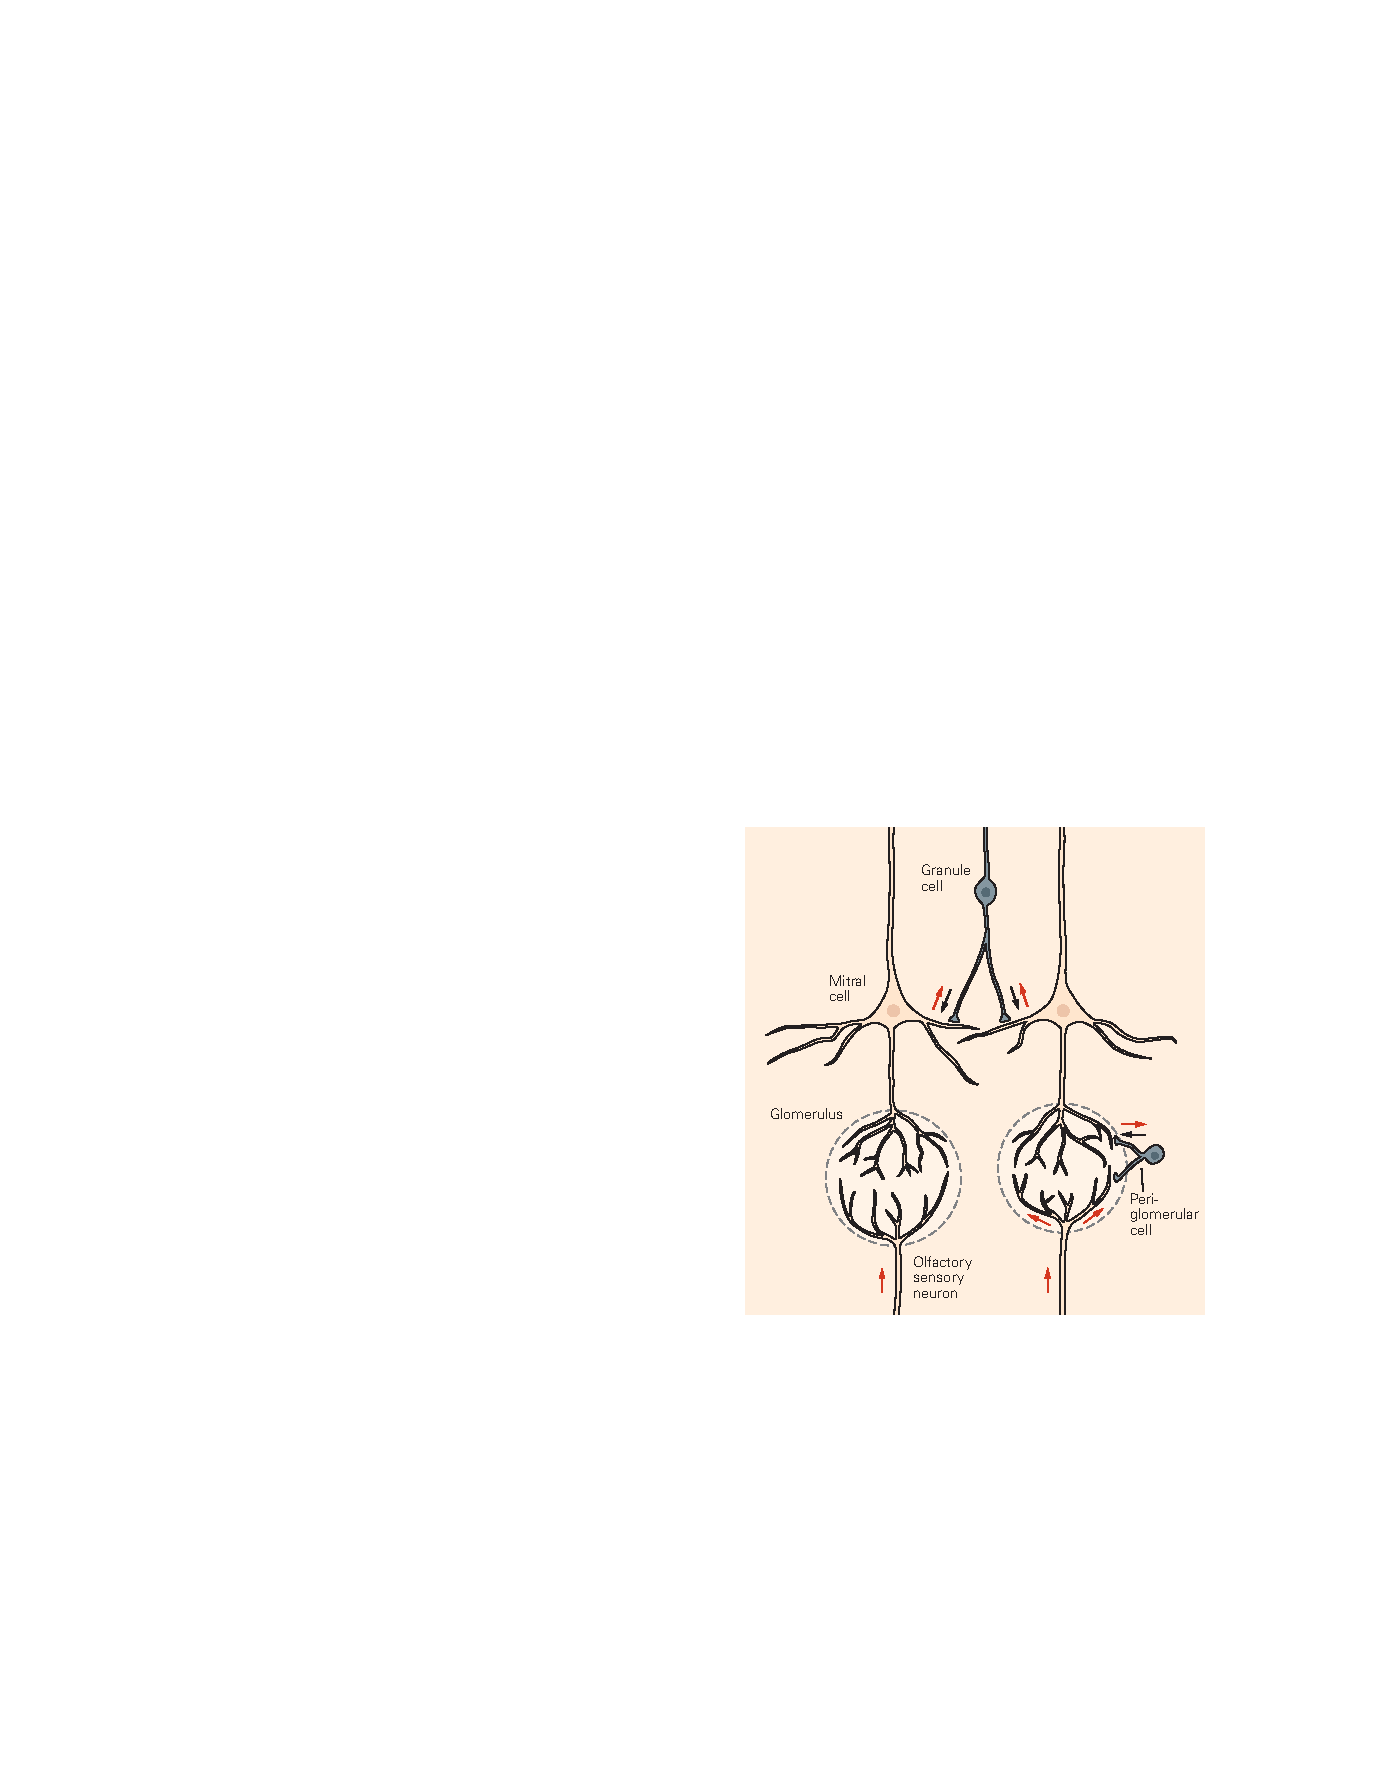
\includegraphics[width=0.5\linewidth]{chap29/fig_29_6}
	\caption{嗅球中间神经元。
		除了兴奋性\textit{僧帽细胞}和簇状中继神经元外,\textit{嗅球}还含有抑制性中间神经元。
		在每个肾小球内,\textit{$\gamma$-氨基丁酸能}球周细胞的树突接收来自嗅觉感觉神经元的兴奋性输入,并与\textit{僧帽细胞}和簇状中继神经元的初级树突形成相互突触,表明可能在信号修饰中发挥作用。
		嗅球深处的\textit{$\gamma$-氨基丁酸能}颗粒细胞的树突与中继神经元的次级树突具有相互兴奋抑制突触,并且被认为向中继神经元提供负反馈,从而形成气味反应\cite{haberly1998synaptic}。}
	\label{fig:29_6}
\end{figure}



嗅觉感觉神经元的轴突以及每个\textit{僧帽细胞}和簇状中继神经元的初级树突终止于单个肾小球。
在每个肾小球中,数千个感觉神经元的轴突会聚在大约 40 到 50 个中继神经元的树突上。
这种收敛导致传递嗅觉信号的神经元数量减少了大约 100 倍。


嗅球中感觉信息的组织与上皮组织截然不同。
虽然具有相同气味受体的嗅觉感觉神经元随机散布在一个上皮区,但它们的轴突通常会聚在特定位置的两个肾小球中,一个位于嗅球的两侧(图~\ref{fig:29_7}C)。
每个肾小球,以及与其相连的每个\textit{僧帽细胞}和簇状中继神经元,仅接收来自一种气味受体的输入。
结果是来自不同气味受体的感觉输入的精确排列,个体之间的感觉输入是相似的。


\begin{figure}[htbp]
	\centering
	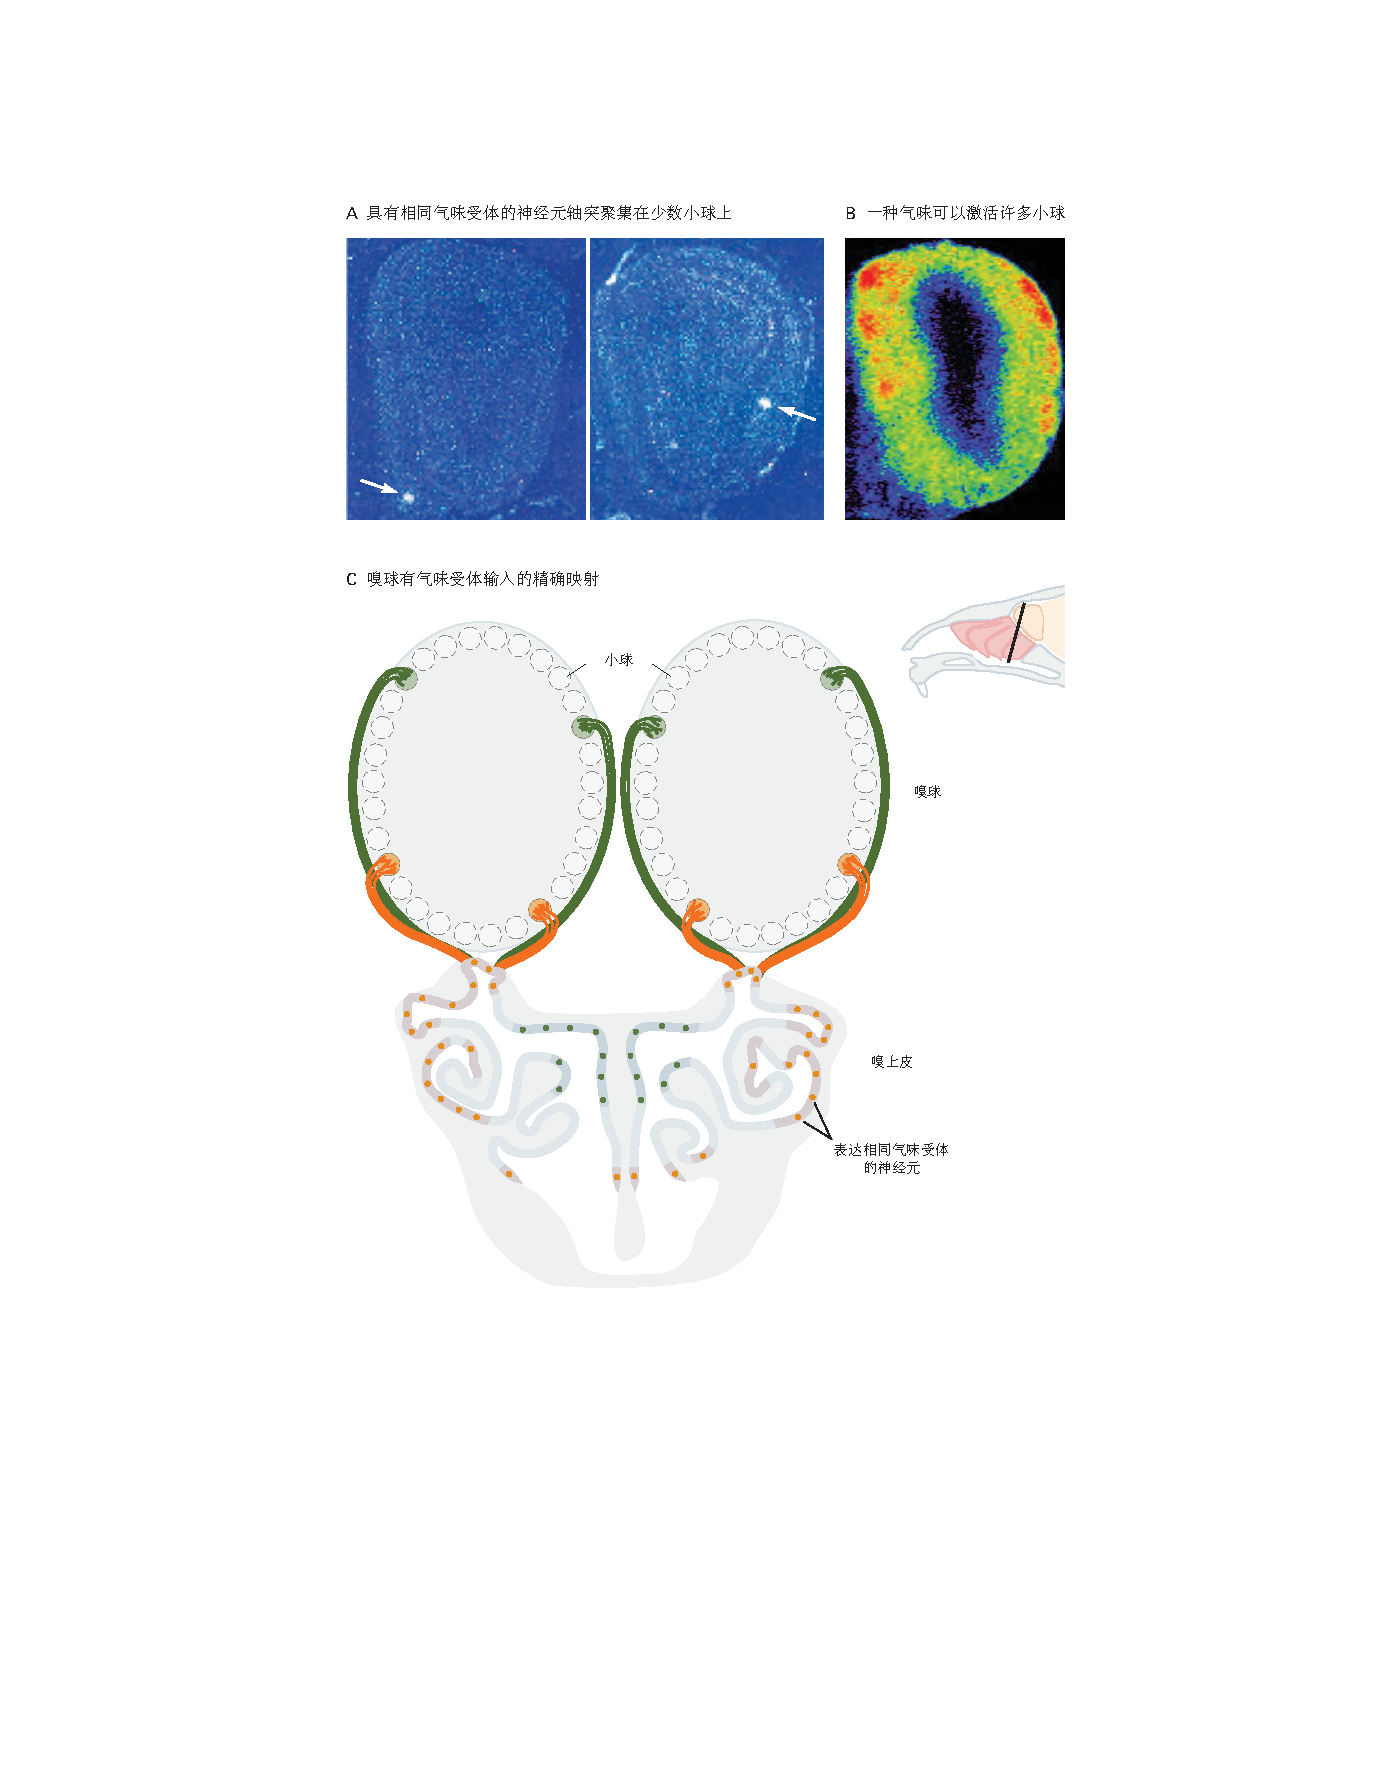
\includegraphics[width=0.7\linewidth]{chap29/fig_29_7}
	\caption{嗅球中的气味反应。
		\textbf{A.} 具有相同气味受体类型的感觉神经元的轴突通常只聚集在两个肾小球中,一个在嗅球的每一侧。
		在这里,一种气味受体基因特异性探针标记了小鼠嗅球内侧(左)和外侧(右)的肾小球。
		探针与存在于这些冠状切片中感觉轴突中的受体信使\textit{核糖核酸}杂交\cite{ressler1994information}。
		\textbf{B.} 一种气味通常会激活来自不同受体的多个肾小球。
		大鼠嗅球的这一部分显示了在动物暴露于有气味的苯甲酸甲酯后在多个焦点(红色)摄取放射性标记的 2-脱氧葡萄糖。
		标记的病灶对应于嗅球不同位置的众多肾小球\cite{johnson2005interactions}。
		\textbf{C.} 嗅球具有气味受体输入的精确映射,因为每个肾小球仅专用于一种类型的受体。
		两个嗅球中的地图是双边对称的,并且在个体之间几乎相同。
		每个灯泡的内侧和外侧的贴图相似,但沿背腹轴和前后轴略微移位。}
	\label{fig:29_7}
\end{figure}


因为每种气味剂都被受体类型的独特组合所识别,所以每种气味剂也会激活嗅球中特定的肾小球组合(图~\ref{fig:29_7}B)。
同时,正如一种气味受体识别多种气味一样,一个肾小球——或一个给定的\textit{僧帽细胞}或簇状细胞——被不止一种气味激活。
由于嗅球中受体输入的模式几乎是刻板的,由个体气味引起的肾小球激活模式在所有个体中都是相似的,并且在两个相邻的球中是双侧对称的。


嗅球中的这种感觉信息组织可能在两个方面具有优势。
首先,来自数千个具有相同气味受体类型的感觉神经元的信号总是会聚在相同的几个肾小球上,嗅球中的中继神经元可以优化对低浓度气味剂的检测。
其次,尽管具有相同受体类型的嗅觉感觉神经元分散并不断更换,但嗅球中输入的排列保持不变。
因此,大脑中气味剂的神经编码会随着时间的推移而保持不变,从而确保可以在多年后识别出以前遇到的气味剂。


一个未解之谜是具有相同类型受体的嗅觉感觉神经元的所有轴突如何指向相同的肾小球。
使用转基因小鼠的研究表明,气味受体本身以某种方式决定了轴突的目标,但尚不清楚它是如何做到这一点的。


感觉信息在被转发到嗅觉皮层之前在嗅球中被处理并可能被提炼。
每个肾小球都被球周中间神经元包围,这些中间神经元接收来自感觉轴突的兴奋性输入,并与该肾小球和可能相邻的肾小球中的\textit{僧帽细胞}和簇状细胞树突形成抑制性树突突触。
因此,肾小球周围神经元可能在信号调制中起作用。
此外,嗅球深处的颗粒细胞中间神经元向\textit{僧帽细胞}细胞和簇状细胞提供负反馈。
颗粒细胞中间神经元被\textit{僧帽细胞}和簇状细胞的基底树突兴奋,进而抑制那些中继神经元和其他与之相连的神经元。 
这些连接提供的横向抑制被认为会抑制来自肾小球的信号,并传递仅对气味反应微弱的神经元,从而在重要和不相关的感觉信息传输到皮层之前加强对比。


信号细化的其他潜在来源是从嗅觉皮层、基底前脑(对角带的水平肢)和中脑(蓝斑和中缝核)到嗅球的逆行投射。
这些连接可以根据动物的生理或行为状态调节嗅球输出。 
例如,当动物饥饿时,一些离心投射可能会增强对食物香气的感知。


\subsection{嗅球向嗅觉皮层传递信息}

\textit{僧帽细胞}的轴突和嗅球的簇状中继神经元通过外侧嗅束投射到嗅觉皮层(图~\ref{fig:29_8} 和图~\ref{fig:29_1})。
嗅皮层,粗略地定义为接收来自嗅球的直接投射的那部分皮层,包括多个解剖学上不同的区域。
六个主要区域是前嗅核,它通过前连合的一部分连接两个嗅球;
杏仁核的前外侧皮层核;
嗅结节; 内嗅皮层的一部分;
梨状皮层是最大的,被认为是主要的嗅觉皮层区域。


\begin{figure}[htbp]
	\centering
	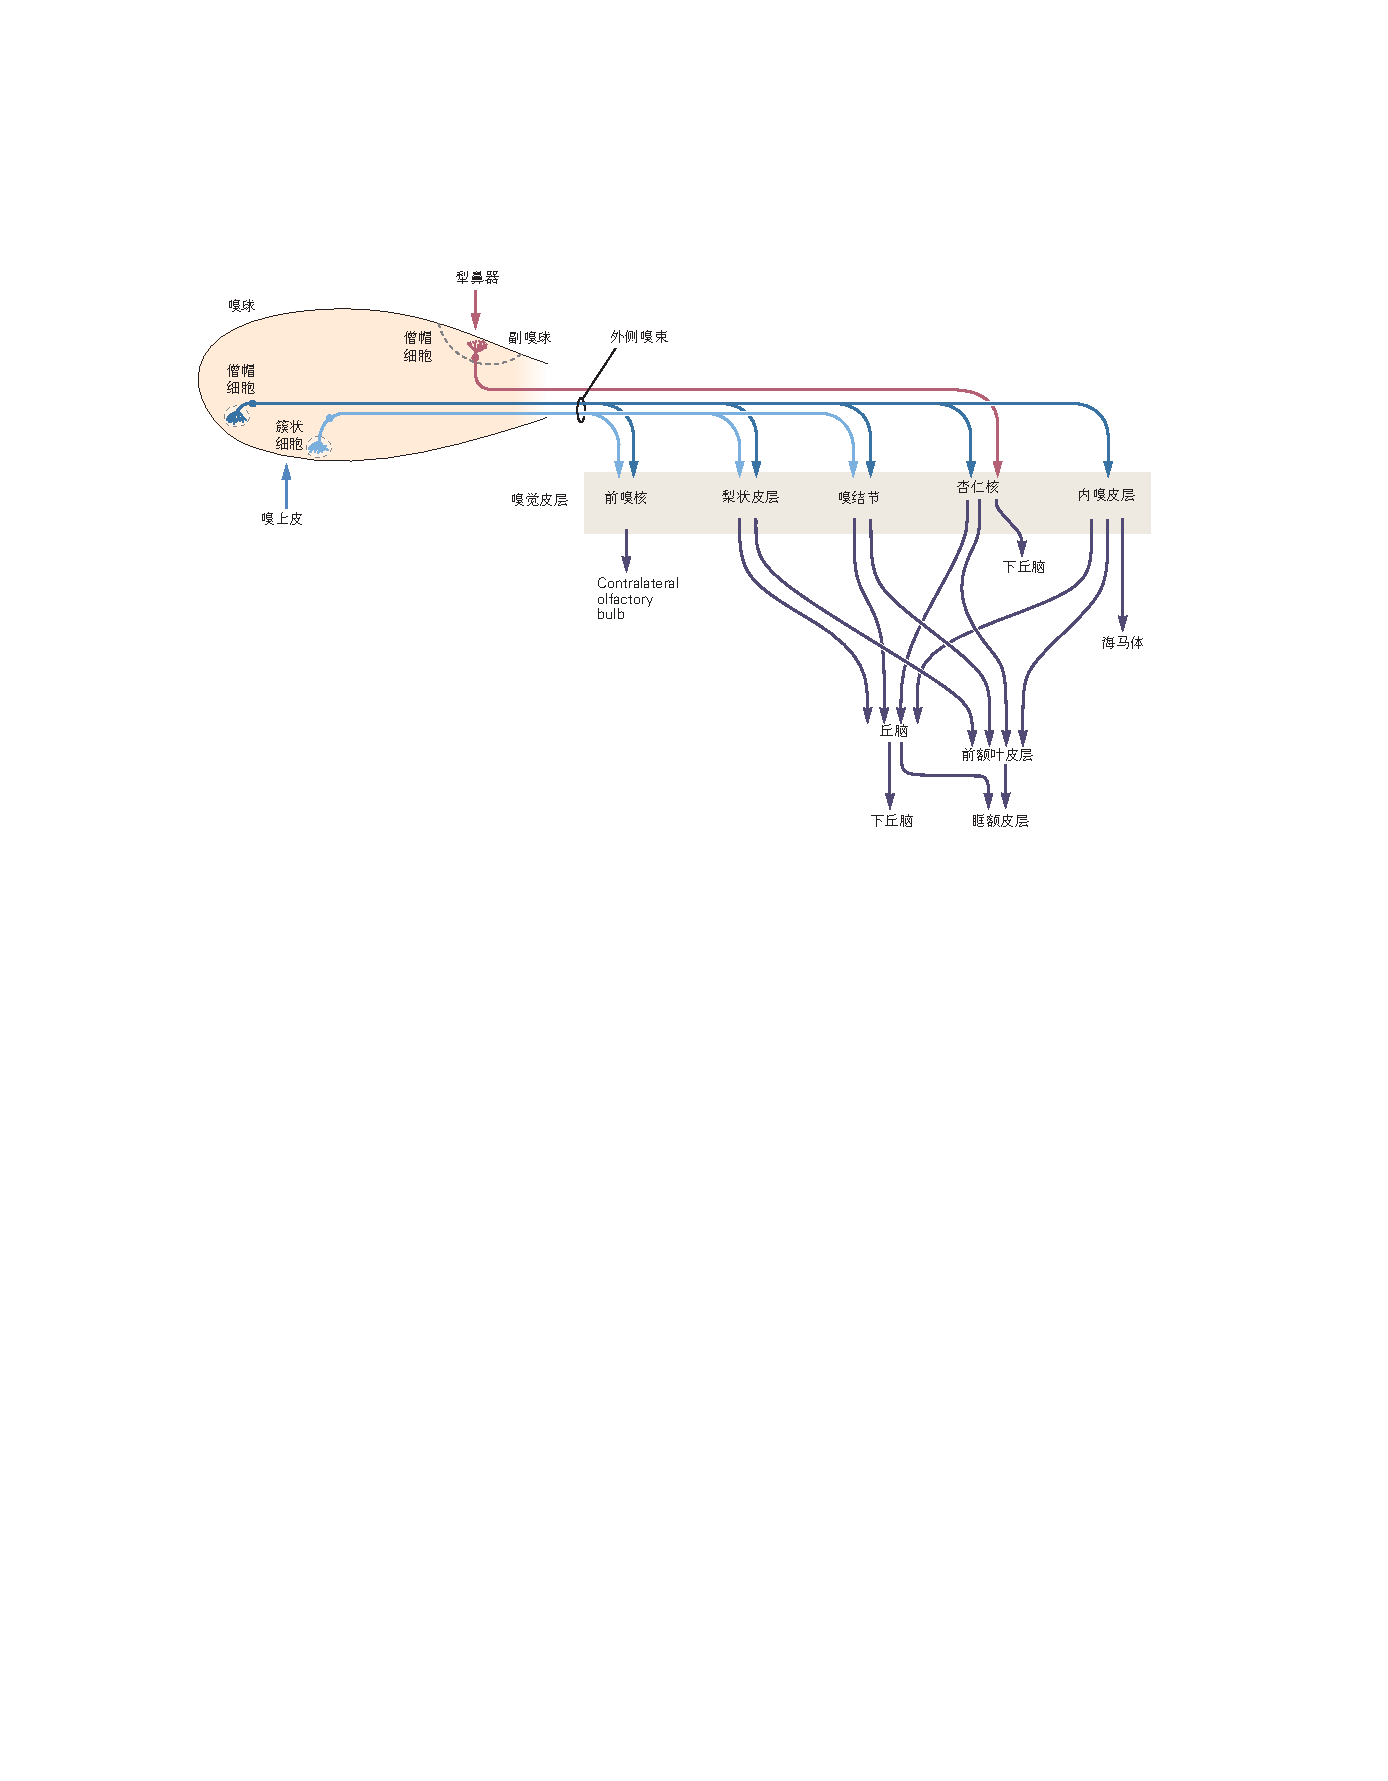
\includegraphics[width=0.9\linewidth]{chap29/fig_29_8}
	\caption{嗅觉皮层的传入通路。
		嗅球的\textit{僧帽细胞}和簇状中继神经元的轴突通过\textit{外侧嗅束}投射到\textit{嗅觉皮层}。
		嗅觉皮层由许多不同的区域组成,其中最大的是梨状皮层。
		从这些区域,嗅觉信息直接或通过丘脑间接传输到其他大脑区域。
		目标包括被认为对气味辨别很重要的新皮层的额叶和眶额区域,以及可能参与对气味的情绪和生理反应的杏仁核和下丘脑。
		辅助嗅球中的\textit{僧帽细胞}细胞投射到杏仁核的特定区域,将信号传递到下丘脑。}
	\label{fig:29_8}
\end{figure}


不同嗅觉皮层区域的功能在很大程度上是未知的。
然而,梨状皮层被认为对气味学习很重要。
最近的研究表明,后外侧皮层杏仁核可能在先天吸引力和恐惧行为中起作用,而杏仁核-梨状过渡区是一个较小的嗅觉皮层区,它在应激激素对鼻子中检测到的捕食者气味的反应中起作用。


在梨状皮层中,嗅球\textit{僧帽细胞}和簇状细胞的轴突离开外侧嗅束,与锥体神经元(皮层的投射神经元)形成兴奋性谷氨酸能突触。
锥体神经元活动似乎受到来自局部 GABAergic 中间神经元的抑制性输入以及来自相同和其他嗅觉皮层区域和对侧梨状皮层中其他锥体神经元的兴奋性输入的调节。
梨状皮层还接收来自调节大脑区域的离心输入,这表明它的活动可以根据生理或行为状态进行调整。
最后,嗅觉皮层投射到嗅球,提供另一种可能的信号调制方式。


与嗅球中继神经元一样,单个锥体神经元可以被一种以上的气味激活。
然而,被特定气味激活的锥体神经元分散在梨状皮层中,这种排列不同于嗅球。
嗅球不同部位的\textit{僧帽细胞}细胞可以将轴突投射到梨状皮层的同一亚区,进一步表明嗅球中高度组织的气味受体输入图并没有在皮层中重现。



\subsection{嗅觉皮层的输出到达更高的皮层和边缘区域}

嗅觉皮层中的锥体神经元通过丘脑将信息间接传递到眶额叶皮层,并直接传递到额叶皮层。
这些通往更高皮层区域的通路被认为在气味辨别中很重要。
事实上,眶额皮层受损的人无法辨别气味。
有趣的是,眶额皮层中的记录表明该区域的一些单个神经元接收多模式输入,例如对香蕉的气味、视觉或味道做出反应。


嗅觉皮层的许多区域也将信息传递到与情绪相关的杏仁核的非嗅觉区域,以及控制食欲等基本驱动力以及许多先天行为的下丘脑。
这些边缘区域被认为在气味的情感和动机方面以及气味剂的许多行为和生理影响中发挥作用。
在动物中,它们可能在对捕食者的气味或在\textit{嗅上皮}细胞中检测到的信息素的刻板行为和生理反应的产生中起重要作用。



\subsection{人类的嗅觉敏锐度各不相同}

人类之间的嗅觉敏锐度可能相差高达 1是千倍,即使在没有明显异常的人之间也是如此。
最常见的嗅觉异常是特异性嗅觉丧失。
患有特定嗅觉缺失症的人对特定气味的敏感性降低,尽管对其他气味的敏感性似乎正常。
对某些气味剂的特定嗅觉缺失很常见,少数发生在 1\% 到 20\% 的人身上。
例如,在一项研究中,12\% 的测试个体表现出对麝香的特定嗅觉丧失。
最近的研究表明,特定气味受体基因的突变可能会导致特定的嗅觉缺失。


更罕见的嗅觉异常,例如全身性嗅觉丧失(完全没有嗅觉)或嗅觉减退(嗅觉减退),通常是短暂的,可由呼吸道感染引起。
慢性嗅觉丧失或嗅觉减退可由感染引起的\textit{嗅上皮}细胞损伤引起;
来自特定疾病,例如帕金森病;
或来自头部外伤,通过筛板中的孔切断嗅觉神经,然后被疤痕组织阻塞。
令人厌恶的气味(恶臭)的嗅觉幻觉可能是癫痫发作的结果。



\section{气味引发特征性先天行为}

\subsection{在两个嗅觉结构中检测到信息素}

在许多动物中,嗅觉系统不仅可以检测气味,还可以检测信息素,即从动物身上释放并影响同一物种成员的行为或生理的化学物质。
信息素在多种哺乳动物中发挥着重要作用,尽管它们尚未在人类中得到证实。
一些信息素通常包含在尿液或腺体分泌物中,可调节生殖激素的水平或刺激性行为或攻击性。
信息素由两个独立的结构检测:鼻\textit{嗅上皮}细胞,检测气味;犁鼻器,一种辅助嗅觉器官,被认为专门用于检测信息素和其他动物线索。


犁鼻器存在于许多哺乳动物中,但不存在于人类中。
它是鼻中隔中的管状结构,具有通向鼻腔的管道和一个衬有感觉上皮细胞的内壁。
犁鼻器上皮细胞中的感觉神经元产生的信号遵循不同的途径。
它们主要通过辅助嗅球到达内侧杏仁核和后内侧皮层杏仁核,并从那里到达下丘脑。


犁鼻器中的感觉检测不同于嗅上皮中的感觉检测。
犁鼻器有两个不同的化学感受器家族,即 V1R 和 V2R 家族。
在小鼠中,每个家庭都有100多个成员。
每个受体家族成员之间氨基酸序列的差异表明每个家族可能识别多种不同的配体。
与气味受体一样,V1R 和 V2R 受体具有典型的 G 蛋白偶联受体的七个跨膜结构域。 
V2R 受体与 V1R 和气味受体的不同之处在于在 N 末端有一个大的细胞外结构域(图~\ref{fig:29_9} A)。
通过类比具有相似结构的受体,配体可以在由跨膜结构域组合形成的膜袋中结合 V1R 受体,而与 V2R 受体的结合可能发生在大的细胞外结构域中。
尽管 V1R 受体被认为可以识别挥发性化学物质,但至少一些 V2R 被认为可以识别蛋白质。
这些包括存在于眼泪中的蛋白质信息素、刺激攻击性的小鼠尿蛋白,以及来自猫和老鼠的捕食者蛋白质,它们会刺激小鼠的恐惧。


\begin{figure}[htbp]
	\centering
	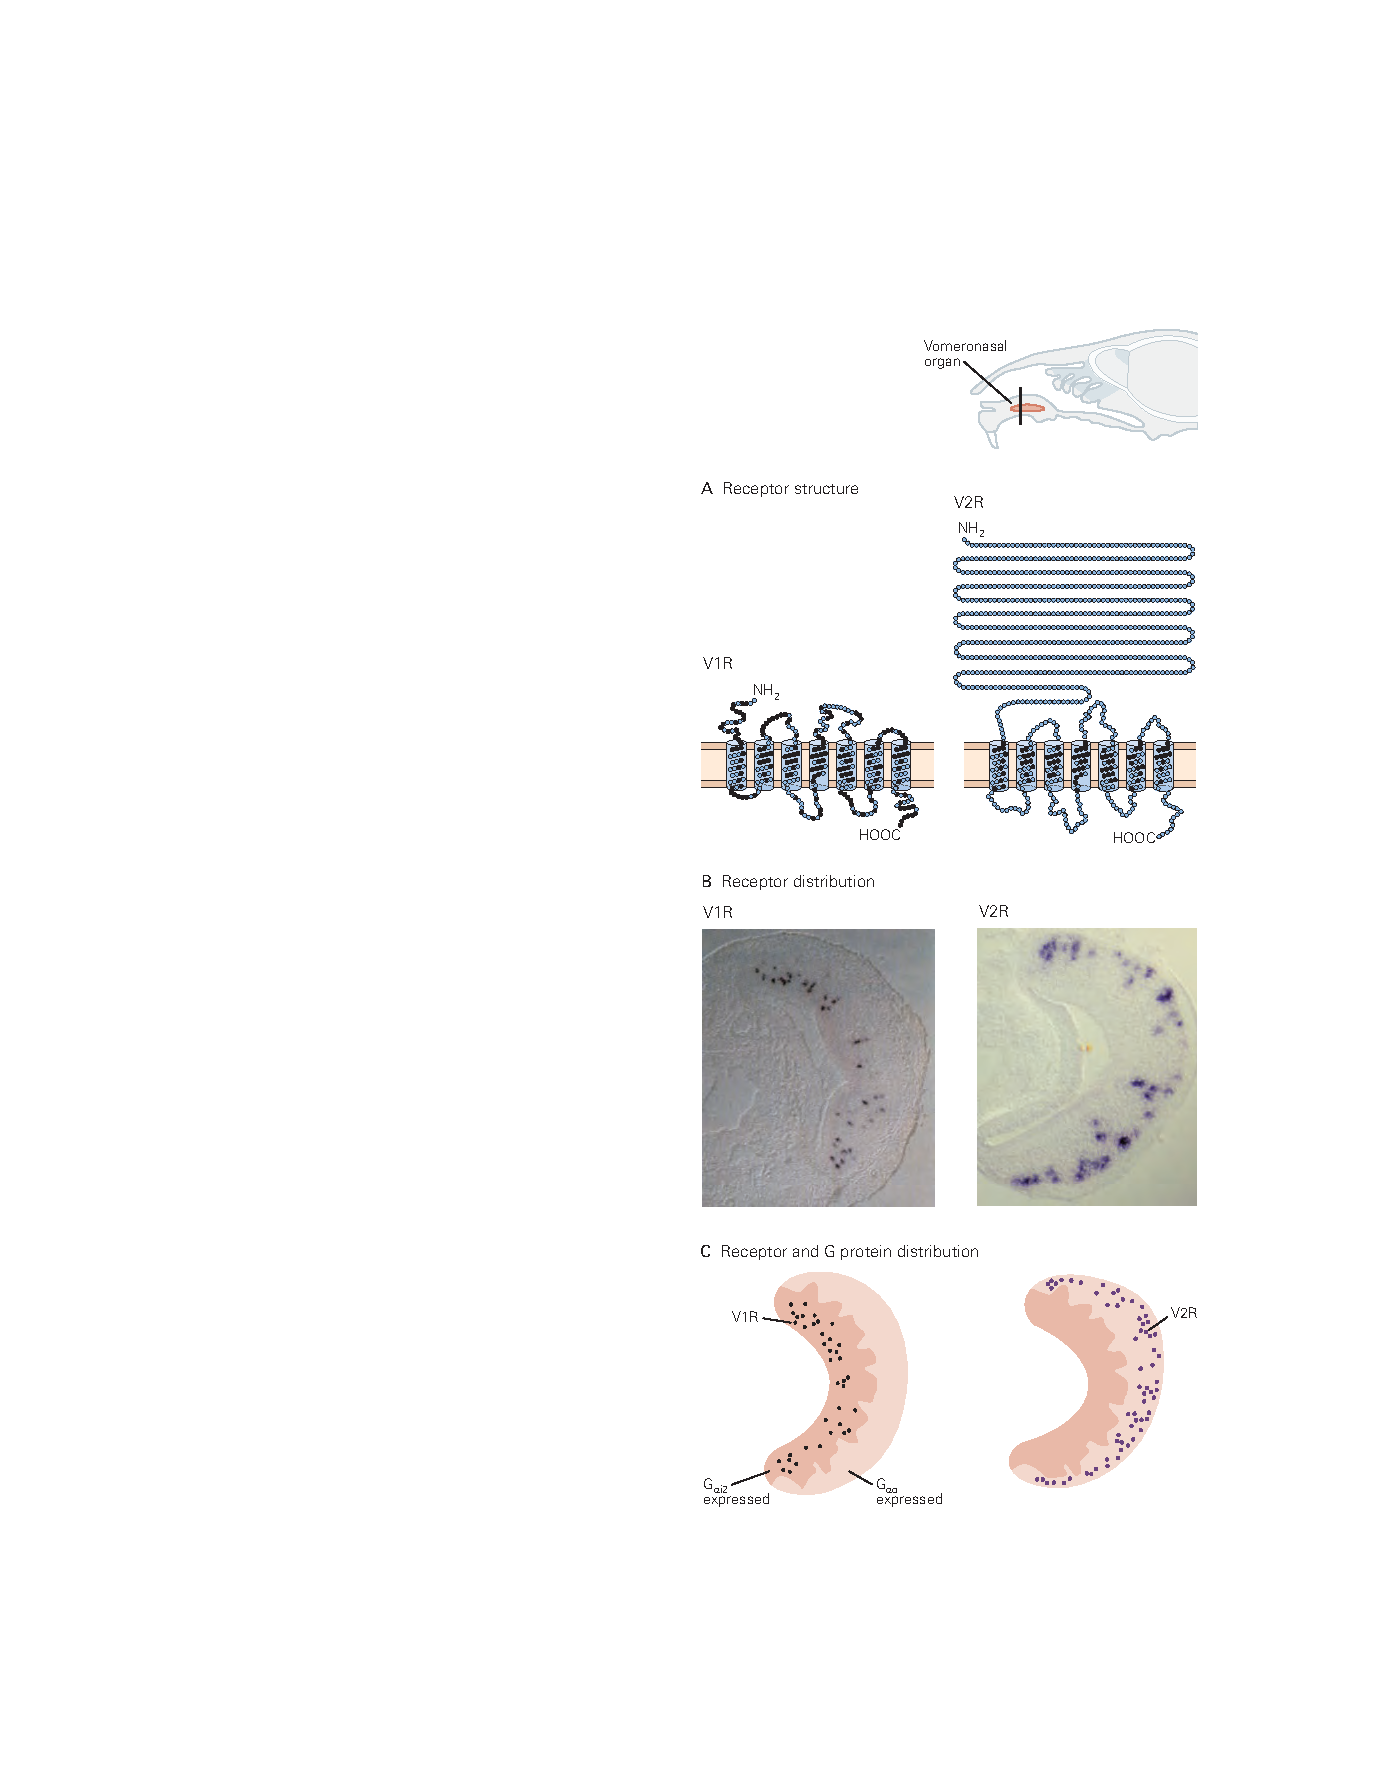
\includegraphics[width=0.75\linewidth]{chap29/fig_29_9}
	\caption{(右)犁鼻器中的候选信息素受体。
		\textbf{A.} V1R 和 V2R 受体家族在犁鼻器中表达。
		在小鼠中,每个家族有 100 多个成员,其蛋白质序列各不相同。
		这两个家族的成员都具有 G 蛋白偶联受体的七个跨膜结构域,但 V2R 受体在 N 末端也有一个大的细胞外结构域,可能是配体结合位点。
		\textbf{B.} 犁鼻器官的切片显示单个 V1R 和 V2R 探针与两个不同区域中的神经元子集杂交。
		\textbf{C.} 这两个区域表达高水平的不同 G 蛋白 $ G_{\alpha i 2} $ 和 $ G_{\alpha o}$ 。}
	\label{fig:29_9}
\end{figure}


V1R 和 V2R 家族在表达不同 G 蛋白的犁鼻器官的不同空间区域中表达(图~\ref{fig:29_9}B、C)。
每个 V1R 或 V2R 基因都在一小部分分散在一个区域的神经元中表达,这种排列类似于\textit{嗅上皮}细胞中气味受体的排列。
与主嗅球相似,具有相同受体类型的犁鼻神经元投射到辅助嗅球中的相同肾小球,尽管每种受体类型的肾小球数量更多,而且它们的分布不如主嗅球中的定型。
除了 V1R 和 V2R 受体外,犁鼻器官还有一个由五种甲酰肽相关受体 (FPR) 组成的家族。
这些受体与检测细菌蛋白的免疫系统 FPR 有关,这引发了人们猜测它们可能在检测同一物种的患病动物方面发挥作用。



\subsection{无脊椎动物嗅觉系统可用于研究气味编码和行为}

由于无脊椎动物具有简单的神经系统,并且经常以刻板的行为对嗅觉刺激做出反应,因此它们有助于理解气味的神经表征与行为之间的关系。


化学感应系统的某些特征在进化过程中高度保守。
首先,所有后生动物都可以使用具有与外部环境接触的纤毛或微绒毛的专门化学感觉神经元来检测各种有机分子。 
其次,气味检测的初始事件是由周围感觉神经元中具有特定表达模式的跨膜受体家族介导的。
嗅觉系统的其他特征因物种而异,反映了动物的选择压力和进化史。


昆虫的主要感觉器官是靠近嘴巴的触角和被称为上颌须肢的附属物(图~\ref{fig:29_10} A)。
哺乳动物有数百万个嗅觉神经元,而昆虫的数量要少得多。
果蝇果蝇中大约有 2,600 个嗅觉神经元,蜜蜂中大约有六万个。


\begin{figure}[htbp]
	\centering
	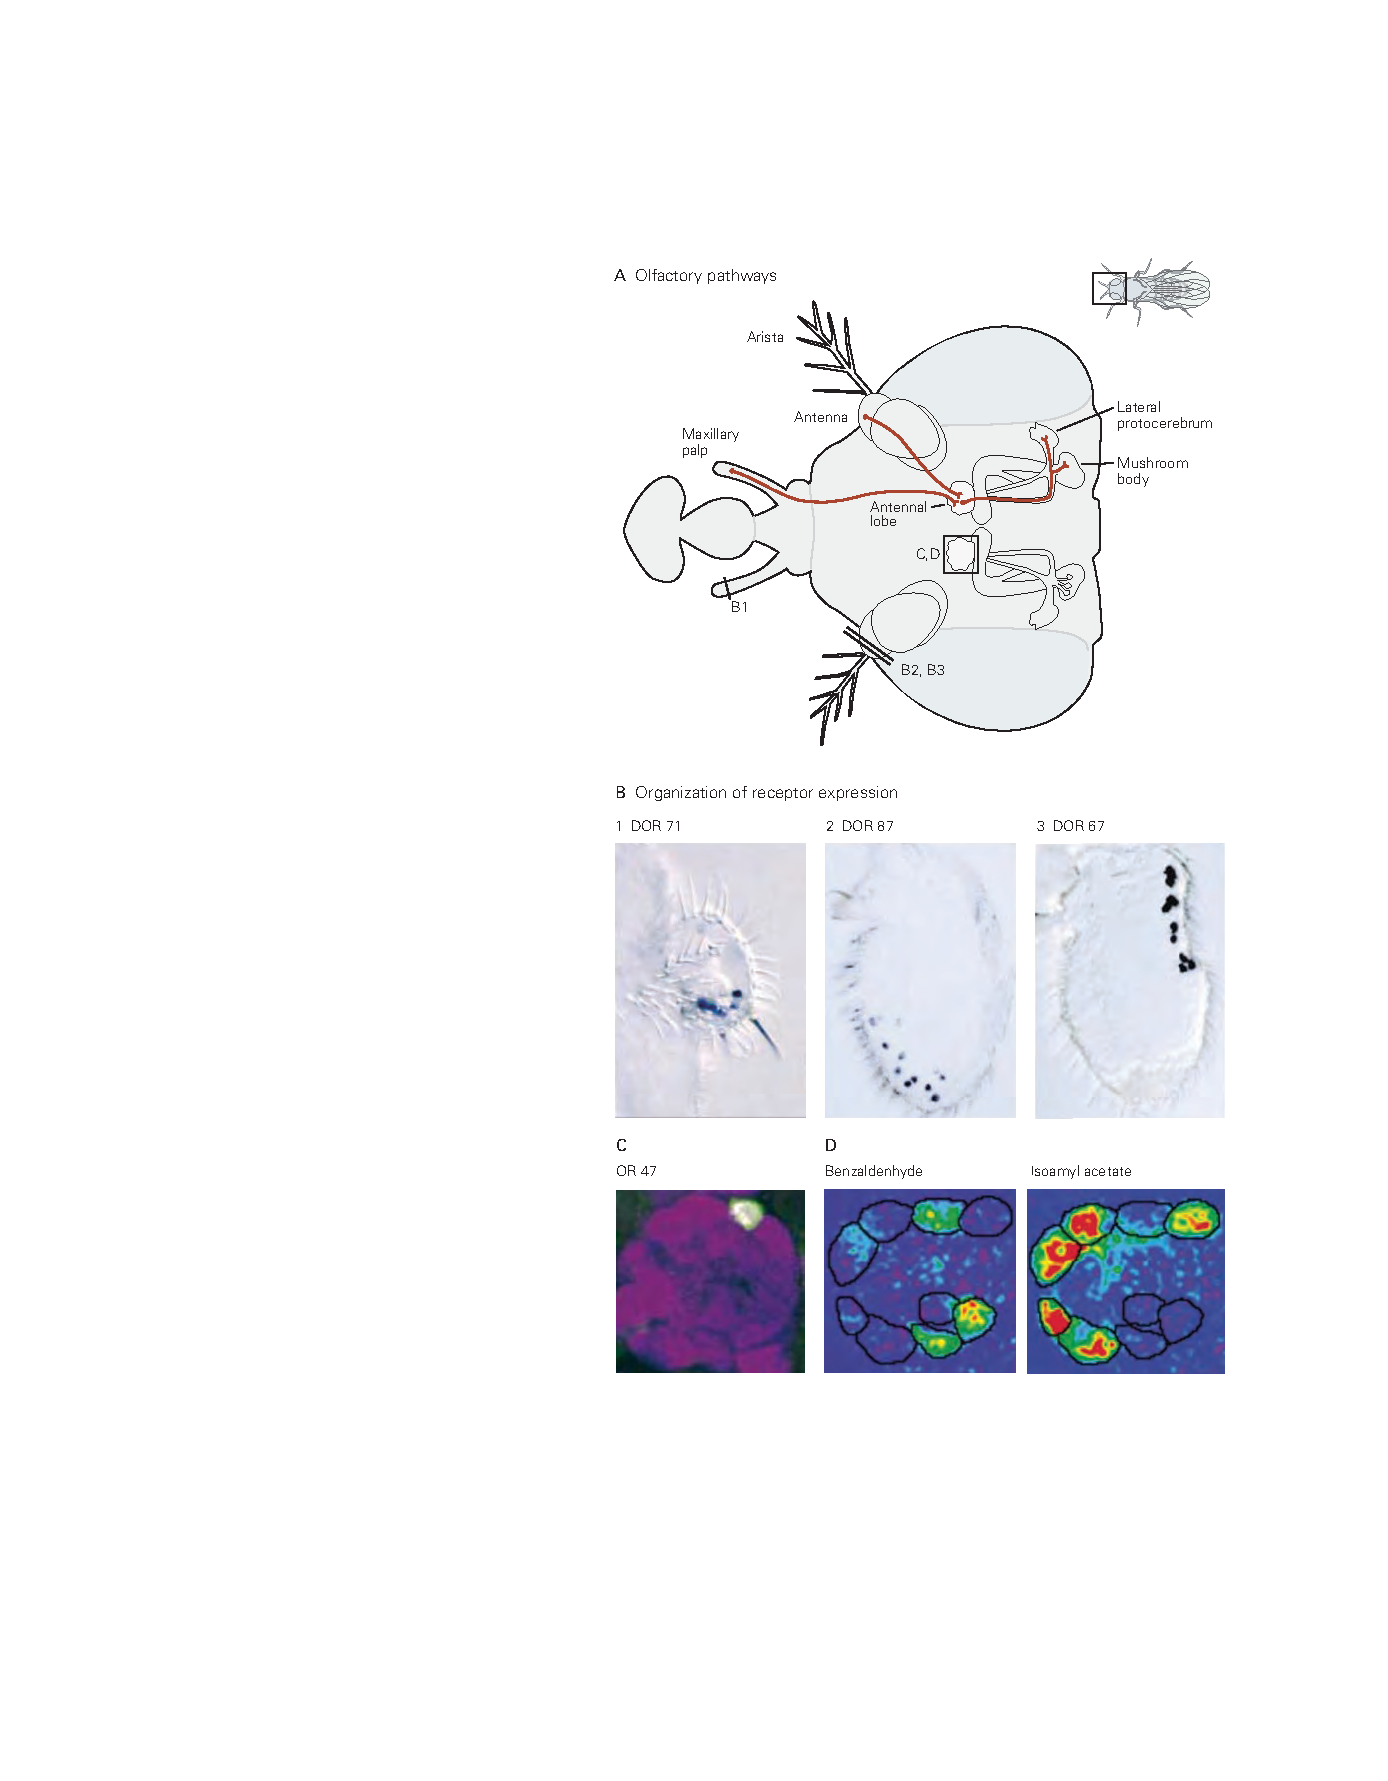
\includegraphics[width=0.8\linewidth]{chap29/fig_29_10}
	\caption{果蝇中从触角到大脑的嗅觉通路。
		\textbf{A.} 触角和上颌触须中具有细胞体和树突的嗅觉神经元的轴突将轴突投射到触角叶。
		触角叶中的投射神经元然后投射到果蝇大脑的两个区域,即蘑菇体和外侧原大脑。
		\textbf{B.} 通过\textit{核糖核酸}原位杂交检测到的表达一种嗅觉受体基因的神经元散布在上颌须 (1) 或天线 (2、3) 中。
		\textbf{C.} 所有表达嗅觉受体基因 OR47 的神经元都聚集在触角叶的肾小球上。
		\textbf{D.} 每种气味都会引起触角叶肾小球子集的生理反应。
		双光子钙成像用于检测气味诱发信号。}
	\label{fig:29_10}
\end{figure}


昆虫气味受体是通过在果蝇基因组中发现多基因受体家族而发现的,这些基因现在也在其他昆虫基因组中进行了检测。
值得注意的是,除了存在许多跨膜结构域外,它们与哺乳动物气味受体几乎没有相似之处。
事实上,昆虫受体似乎具有独立于哺乳动物受体的进化起源,甚至可能不是 G 蛋白偶联受体——这是在所有嗅觉受体系统中观察到的快速进化变化的一个极端例子。
在果蝇中,主要的气味受体家族只有60个基因,而不是脊椎动物的数百个特征基因。
疟疾蚊子冈比亚按蚊和蜜蜂具有相似的数量(85-95 个基因),而切叶蚁具有超过 350 个气味受体基因,这表明昆虫的受体数量存在很大差异。


尽管受体存在分子差异,但果蝇嗅觉系统的解剖结构与脊椎动物非常相似。
每个嗅觉神经元表达一种或有时两种功能性气味受体基因。
表达特定基因的神经元松散地位于天线的一个区域,但散布着表达其他基因的神经元(图~\ref{fig:29_10} B)。
这种分散分布在下一级组织(触角叶)中并非如此。
来自表达一种受体的感觉神经元的轴突会聚在触角叶中的两个不变肾小球上,动物的左右两侧各有一个(图 29–10C)。
这种组织与脊椎动物嗅球中的第一个感觉中继器惊人地相似,也存在于飞蛾、蜜蜂和其他昆虫中。


因为果蝇中只有几十个受体基因,所以有可能表征气味-受体相互作用的整个库,而哺乳动物尚未实现这一目标。
复杂的遗传方法可用于标记和记录表达单个已知气味受体基因的果蝇神经元。
通过用许多受体和气味重复这个实验,气味受体的感受野已经被定义并显示出相当多样化。


在昆虫中,单个气味受体可以检测大量气味,包括化学结构非常不同的气味。
如果只有少数受体可用于检测所有具有生物学意义的气味剂,则“通才”受体对气味剂的广泛识别是必要的。
检测多种气味的单一昆虫受体蛋白可以被一些气味刺激并被其他气味抑制,通常具有不同的时间模式。
传达有关信息素或其他不寻常气味(如二氧化碳)信息的昆虫气味受体子集更具选择性。
因此,每个嗅觉神经元的编码潜能可宽可窄,由传递到其受体的刺激和抑制信号的组合产生。


来自嗅觉神经元的信息被传递到触角叶,在那里表达相同气味受体的感觉神经元会聚到一个肾小球中的少量投射神经元(图~\ref{fig:29_10}A)。
由于果蝇肾小球的位置是固定的,并且具有一种气味受体输入,因此可以描述跨突触的信息转换。
许多嗅觉感觉轴突会聚到少数投射神经元上,导致嗅觉信号的信噪比大大增加,因此投射神经元对气味的敏感度远高于单个嗅觉神经元。
在触角叶内,兴奋性中间神经元将信号分配到远端位置的投射神经元,抑制性中间神经元反馈到嗅觉感觉神经元以抑制它们的输入。
因此,当单个嗅觉神经元的活动被传送到一个肾小球时。 它的活动也分布在整个触角叶,因为它由连接许多肾小球的兴奋性和抑制性局部中间神经元处理。


来自触角叶的投射神经元延伸到更高的大脑中心,称为蘑菇体和外侧原大脑(图~\ref{fig:29_10}A)。
这些结构可能代表嗅觉皮层的昆虫等效物。 蘑菇体是嗅觉联想学习和多模式联想学习的场所;
外侧原脑对于先天嗅觉反应很重要。
在这个阶段,投射神经元与大量的下游神经元形成复杂的联系。
果蝇高级大脑中枢的神经元具有整合来自许多受体的信息的潜力。


\subsection{嗅觉线索引起线虫的刻板行为和生理反应}

线虫蛔虫Caenorhabditis elegans拥有动物界最简单的神经系统之一,整个动物只有 302 个神经元。
其中,32 个是纤毛化学感觉神经元。
由于秀丽隐杆线虫对多种化学物质具有强烈的行为反应,因此它一直是将嗅觉信号与行为联系起来的有用实验动物。
每个化学感觉神经元检测一组特定的化学物质,并且神经元的激活是对这些物质的行为反应所必需的。
特定反应的神经元,例如对特定气味的吸引,在所有个体中都出现在相同的位置。


通过对缺乏检测气味能力(嗅觉缺失)的突变蠕虫进行遗传筛选,阐明了秀丽隐杆线虫嗅觉的分子机制。
挥发性气味二乙酰的 G 蛋白偶联受体从这些筛选中出现(图~\ref{fig:29_11})。
该受体是秀丽隐杆线虫中大约 1,700 个预测的 G 蛋白偶联化学感受器基因之一,是已知基因组中数量最多的化学感受器。
还存在其他种类的化学感应受体;
例如,秀丽隐杆线虫通过检测直接与氧气结合的可溶性鸟苷酸环化酶来间接感知外部氧气水平。
由于有如此多的化学感受器,线虫能够非常灵敏地识别各种各样的气味。
一些化学感觉神经元使用 G 蛋白来调节环鸟苷 3',5'-单磷酸 (cGMP) 和 cGMP 门控通道,这是一种类似于脊椎动物光感受器的信号转导途径。
其他化学感觉神经元通过\textit{瞬时受体电位香草醛受体}通道发出信号,如脊椎动物伤害性神经元。


\begin{figure}[htbp]
	\centering
	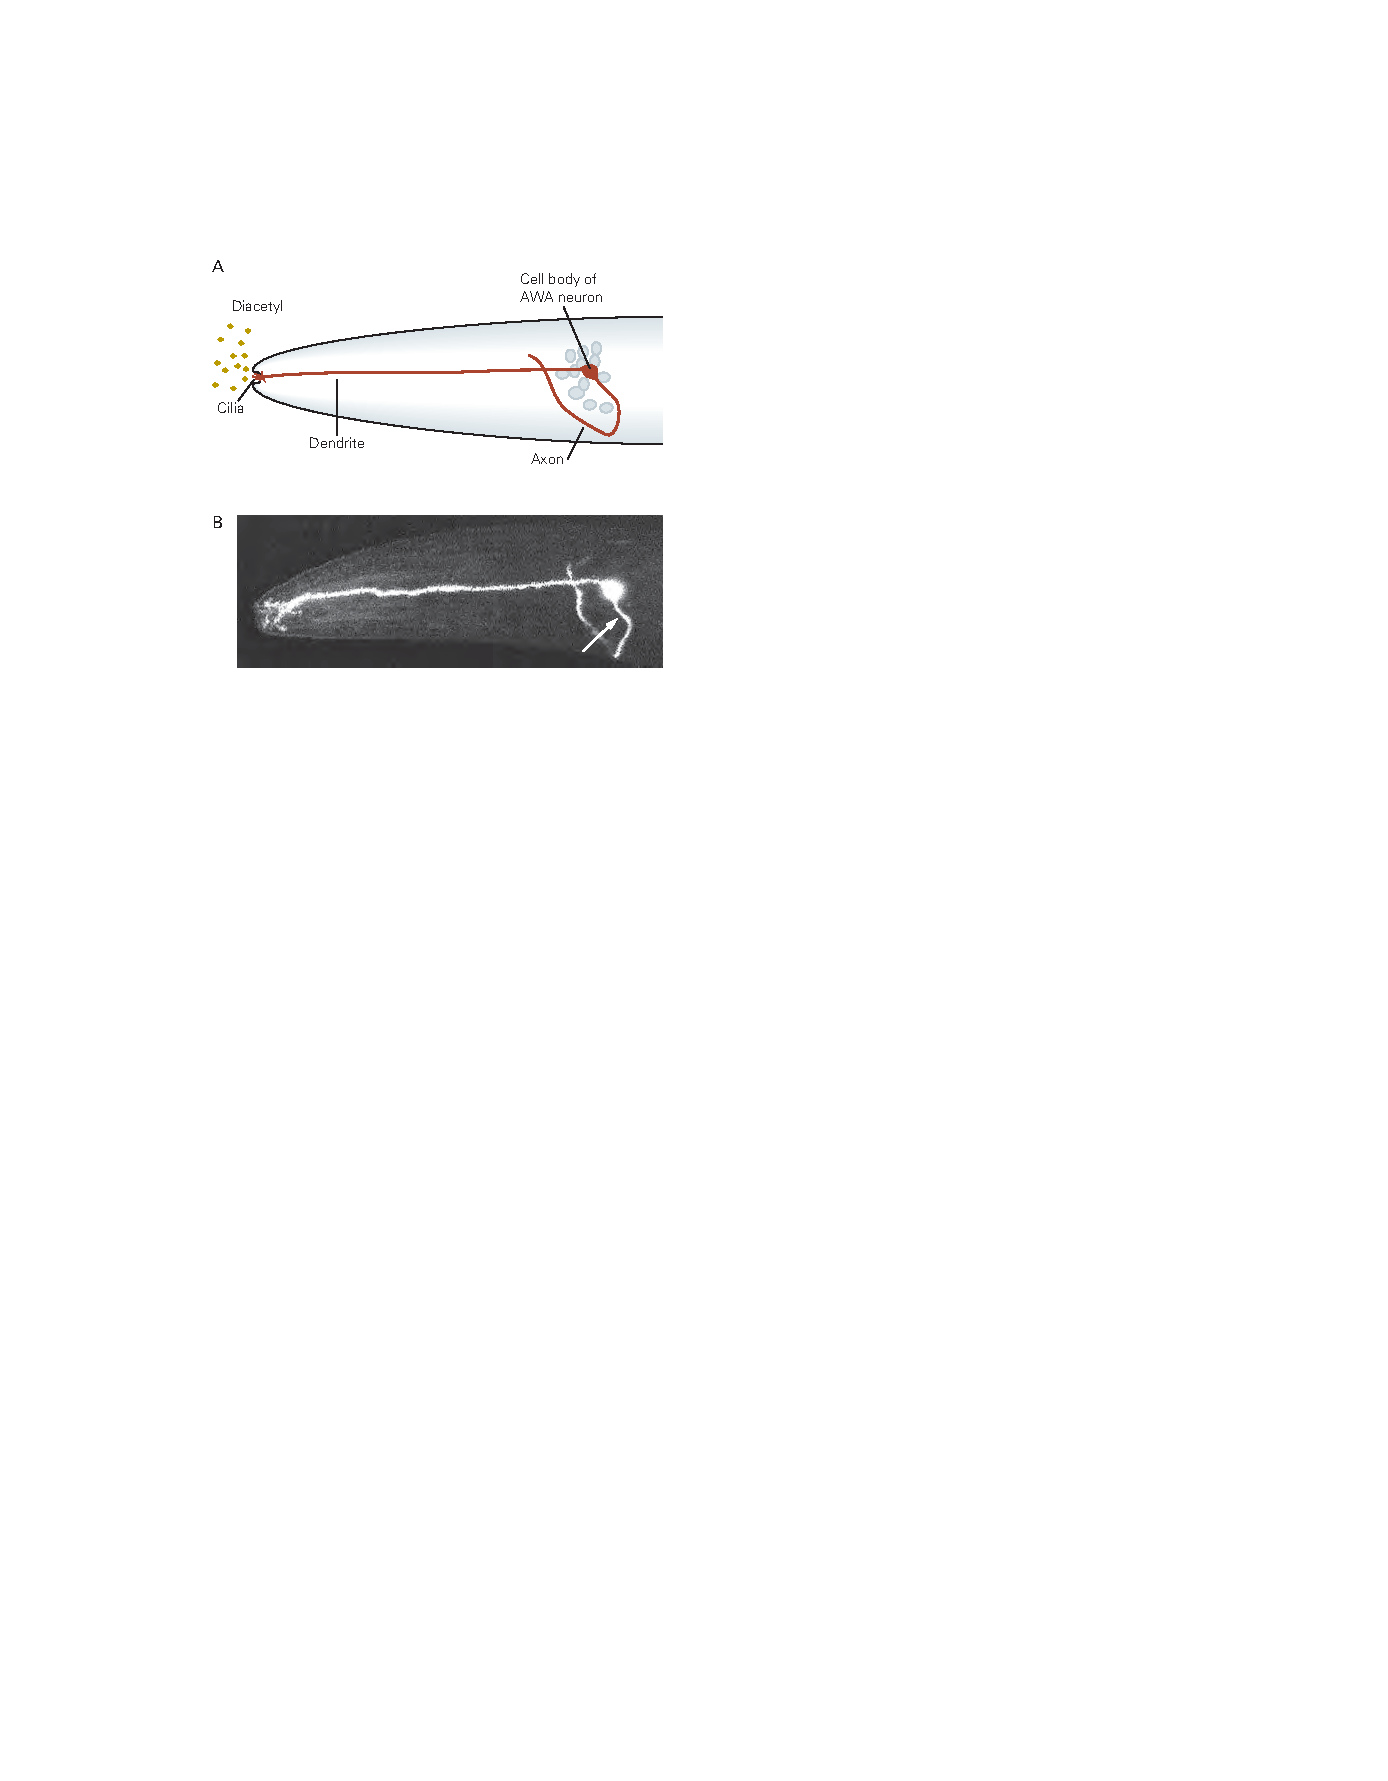
\includegraphics[width=0.8\linewidth]{chap29/fig_29_11}
	\caption{秀丽隐杆线虫中双乙酰的受体。
		\textbf{A.} 蠕虫前端的侧视图显示了 AWA 化学感觉神经元的细胞体和过程。
		树突终止于暴露于环境化学物质的纤毛。
		神经元检测到挥发性化学物质丁二酮;
		odr-10 基因发生突变的动物无法感知双乙酰。
		\textbf{B.} odr-10 基因仅在 AWA 神经元中有活性。
		此处的显微照片显示标记为与荧光报告蛋白融合的基因产物;
		箭头表示神经元的轴突。}
	\label{fig:29_11}
\end{figure}


在脊椎动物和昆虫中观察到的“一个神经元,一个受体”原理并不适用于线虫,因为神经元的数量远小于受体的数量。
每个化学感受器基因通常仅在一对化学感受神经元中表达,但每个神经元表达许多受体基因。
C. elegans 神经系统的小尺寸限制了嗅觉计算。
例如,单个神经元对多种气味有反应,但只有当不同的初级感觉神经元感知到气味时,才能有效地区分气味。


气味检测和行为之间的关系已经通过基因操作在秀丽隐杆线虫中进行了探索。
例如,双乙酰通常对蠕虫有吸引力,但当双乙酰受体在通常感知驱虫剂的嗅觉神经元中通过实验表达时,动物反而被双乙酰排斥。
这一观察表明,特定的感觉神经元编码了吸引或排斥的硬连线行为反应,并且“标记线”将特定气味与特定行为联系起来。
类似的想法也出现在小鼠和果蝇味觉系统的遗传操作中,其中甜味和苦味偏好通路由不同组的感觉细胞编码。


嗅觉线索与线虫的生理反应和行为反应有关。
特定的感觉神经元通过 G 蛋白偶联受体检测调节发育的食物和信息素线索。
在信息素水平低和食物充足的情况下,动物会迅速发育到成年,而在信息素水平高和食物稀缺的情况下,动物会停滞在称为 dauer larvae 的长寿幼虫阶段(图 ~\ref{fig:29_12})。
这些感觉神经元的激活最终调节胰岛素信号通路的活性,该通路控制线虫的生理和生长以及寿命。
其他动物的化学感应系统和生理系统是否像线虫一样纠缠在一起,这是一个悬而未决的问题。


\begin{figure}[htbp]
	\centering
	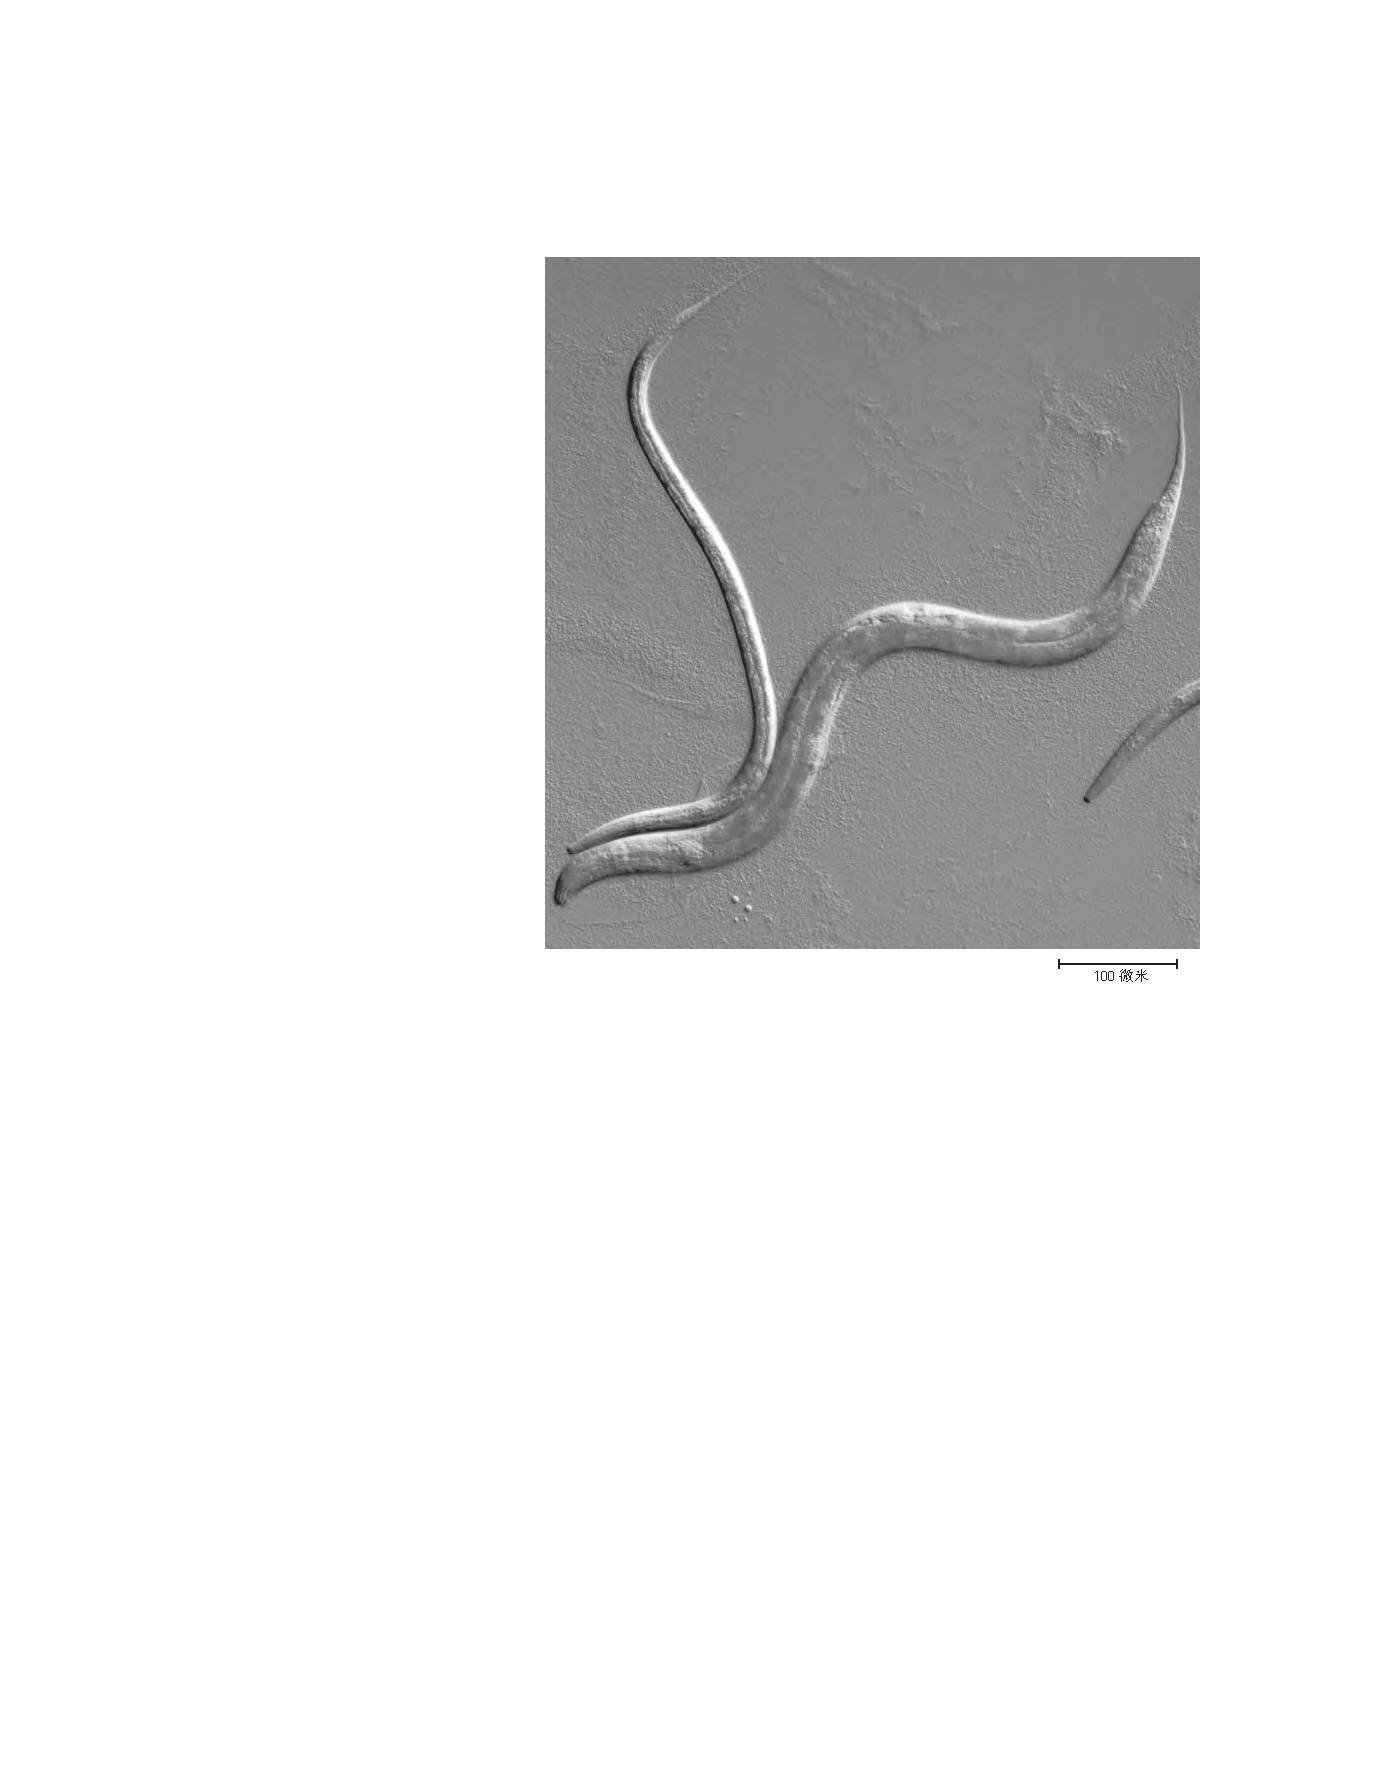
\includegraphics[width=0.6\linewidth]{chap29/fig_29_12}
	\caption{化学感应线索调节秀丽隐杆线虫的发育。
		当暴露于不同的化学感应信号时,两个同龄的幼虫会遵循不同的发育路径。
		在低食物和高人口密度的压力条件下形成的 dauer 幼虫发育成细长的成虫(左)。
		它是一种不进食、不繁殖、抗压的蠕虫。
		相反,在有利于生殖生长的丰富环境中的幼虫发育成正常的成虫(右)。}
	\label{fig:29_12}
\end{figure}



\subsection{嗅觉策略发展迅速}

为什么在哺乳动物、线虫和昆虫中进化出独立的气味受体家族?
与参与其他重要生物过程的基因相比,为什么这些家族的变化如此之快?
答案在于嗅觉与视觉、触觉和听觉等其他感官之间的根本区别。


大多数感官旨在检测具有可靠物理特性的物理实体:光子、压力或声波。
相比之下,嗅觉系统旨在检测无限变化且不符合简单连续特性的有机分子。
此外,检测到的有机分子是由其他生物体产生的,这些生物体的进化速度远远超过光、压力和声音的世界。


今天存在的所有动物的共同祖先都有一个古老的嗅觉系统。
那个祖先生活在海洋中,在那里它产生了哺乳动物、昆虫和线虫的不同谱系。
这三个动物门在门分化后数亿年才登陆陆地。
每个门独立地修改其嗅觉系统以检测空气中的气味,从而导致受体多样化。


考虑在过去 2 亿年中进化的双翅目和膜翅目昆虫的自然史,有助于解释气味受体的快速多样化。
这些昆虫包括为花朵授粉的蜜蜂、以腐烂水果为食的果蝇、死后几分钟内抵达的果蝇,以及捕食活体动物的蚊子。
对这些昆虫的生存很重要的气味物质完全不同,针对这些气味物质调整的受体基因也相应进化。



\section{味觉系统控制味觉}

\subsection{味觉有五种反映基本饮食需求的亚模式}

味觉系统是一种专门用于评估潜在食物来源的化学感觉系统。
它是唯一可以检测食物中糖分和有害化合物的感觉系统,并且是喂养决定的主要驱动力。
与区分数百万种气味的嗅觉系统不同,味觉系统只能识别几个味道类别。


人类和其他哺乳动物可以区分五种基本的味觉品质:甜、苦、咸、酸和鲜味,鲜味是一个日语词,意思是美味,与氨基酸的“咸味”味道有关。
这种有限的味觉可以检测动物的所有基本饮食需求:甜味会吸引富含能量的食物;
苦味警告不要摄入有毒、有害的化学物质;
咸味促进饮食保持适当的电解质平衡;
酸味表示酸性、未成熟或发酵的食物;
umami 表示富含蛋白质的食物。


与碳水化合物和蛋白质的营养重要性一致,甜味和鲜味促味剂都会引起人类天生愉悦的感觉,并且通常是动物的引诱剂。
相比之下,苦味和酸味促味剂会引起人类和动物天生的厌恶反应。


味道通常被认为是风味的同义词。
然而,味觉严格指味觉系统中编码的五种品质,而风味具有丰富多样的品质,源于味觉、嗅觉和体感系统(如质地和温度)输入的多感官整合。



\subsection{味蕾中发生促味剂检测}

促味剂由聚集在味蕾中的味觉感受器细胞检测。
虽然人类的大部分味蕾位于舌头表面,但也有一些位于上颚、咽部、会厌和食道的上三分之一处。


舌头上的味蕾出现在称为乳突的结构中,根据形态和位置,乳突分为三种类型。
位于舌头前三分之二的菌状乳头是钉状结构,顶部有味蕾。
位于舌后缘的叶状乳头和在舌后部区域仅有少数的环状乳头都是被排列有味蕾的凹槽包围的结构(图~\ref{fig:29_13}A)。
在人类中,每个菌状乳头含有一到五个味蕾,而每个叶状乳头和环状乳头可能分别含有数百到数千个味蕾。


\begin{figure}[htbp]
	\centering
	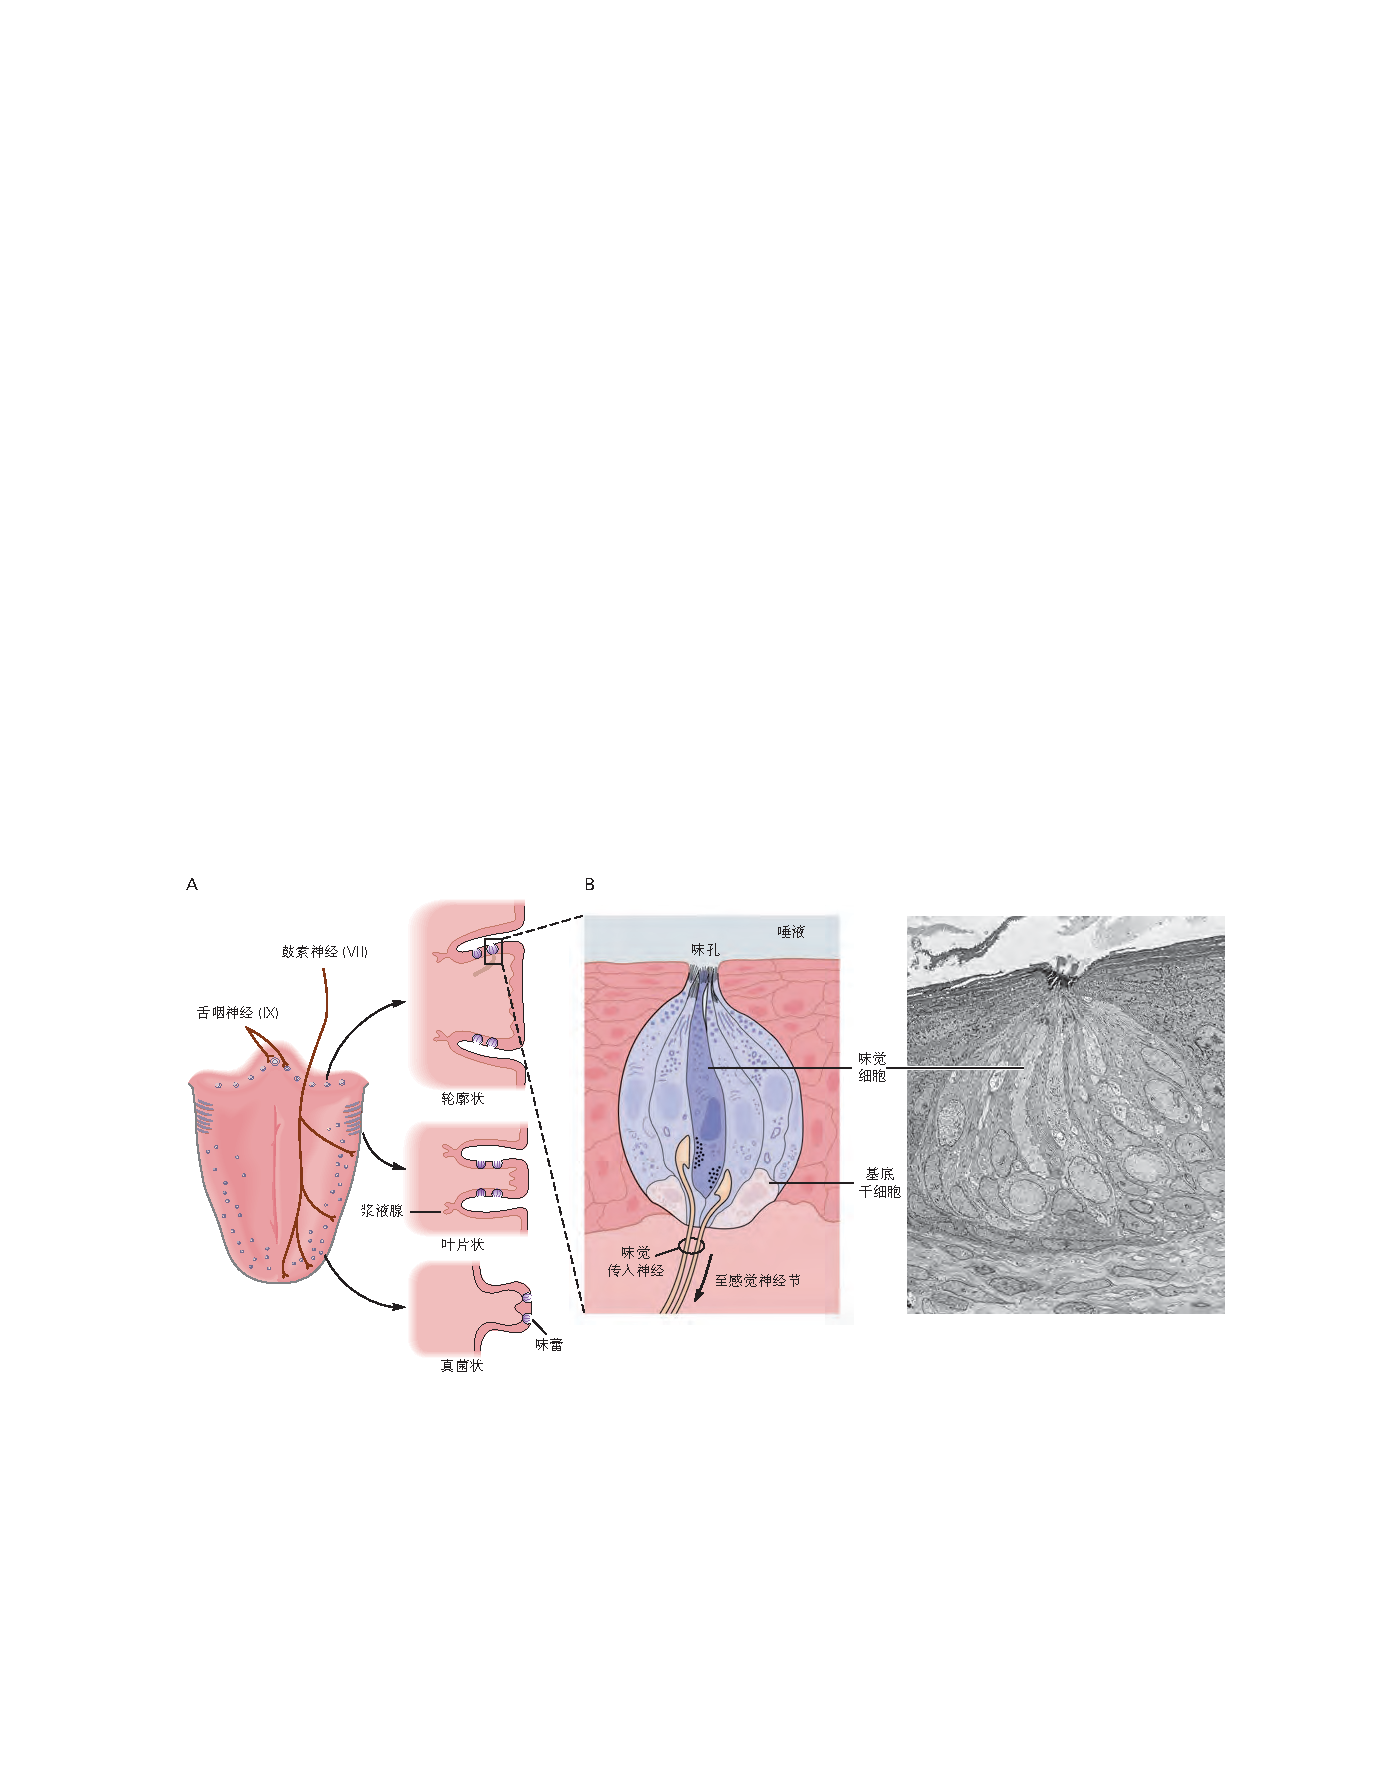
\includegraphics[width=0.10\linewidth]{chap29/fig_29_13}
	\caption{味蕾聚集在舌头上的乳突中。
		\textbf{A.} 三种类型的乳头——环状、叶状和菌状——在舌头上的形态和位置不同,并且分别受鼓索和舌咽神经支配。
		\textbf{B.} 每个味蕾含有 50 到 150 个细长的味觉感受器细胞,以及支持细胞和少量基底干细胞。
		味觉细胞将微绒毛延伸到味孔中,使其能够检测溶解在唾液中的促味剂。
		在其基端,味觉细胞接触味觉神经元,后者将刺激信号传递给大脑。
		扫描电子显微照片显示了兔子叶状乳头中的味蕾。}
	\label{fig:29_13}
\end{figure}


味蕾是嵌入上皮的大蒜状结构。
上皮表面的一个小开口,即味孔,是与促味剂的接触点(图~\ref{fig:29_13}B)。
每个味蕾包含大约 100 个味觉感受器细胞(味觉细胞),这些细长的细胞从味孔延伸到味蕾的基部区域。
味蕾还包含其他被认为具有支持功能的细长细胞,以及基部的少量圆形细胞,被认为是干细胞。
每个味觉细胞都将微绒毛延伸到味孔中,使细胞能够接触上皮表面溶解在唾液中的化学物质。


在其基端,味觉细胞接触味觉感觉神经元的传入纤维,其细胞体位于特定的感觉神经节中(见图~\ref{fig:29_17})。
尽管味觉细胞是非神经性的,但它们与味觉感觉神经元的接触具有化学突触的形态学特征,包括成簇的突触前小泡。
味觉细胞也类似于神经元,因为它们是电兴奋的。
它们具有电压门控的 \ce{Na+}、\ce{K+} 和 \ce{Ca^2+} 通道,能够产生动作电位。
味觉细胞的寿命非常短(数天至数周),并且不断从干细胞群中被替换。
这种转变需要新生的味觉细胞分化以检测五种味觉品质中的一种,并连接到适当的味觉感觉神经元的末端,例如甜味细胞连接到甜味感觉神经元,苦味细胞连接到苦味感觉神经元。


\begin{figure}[htbp]
	\centering
	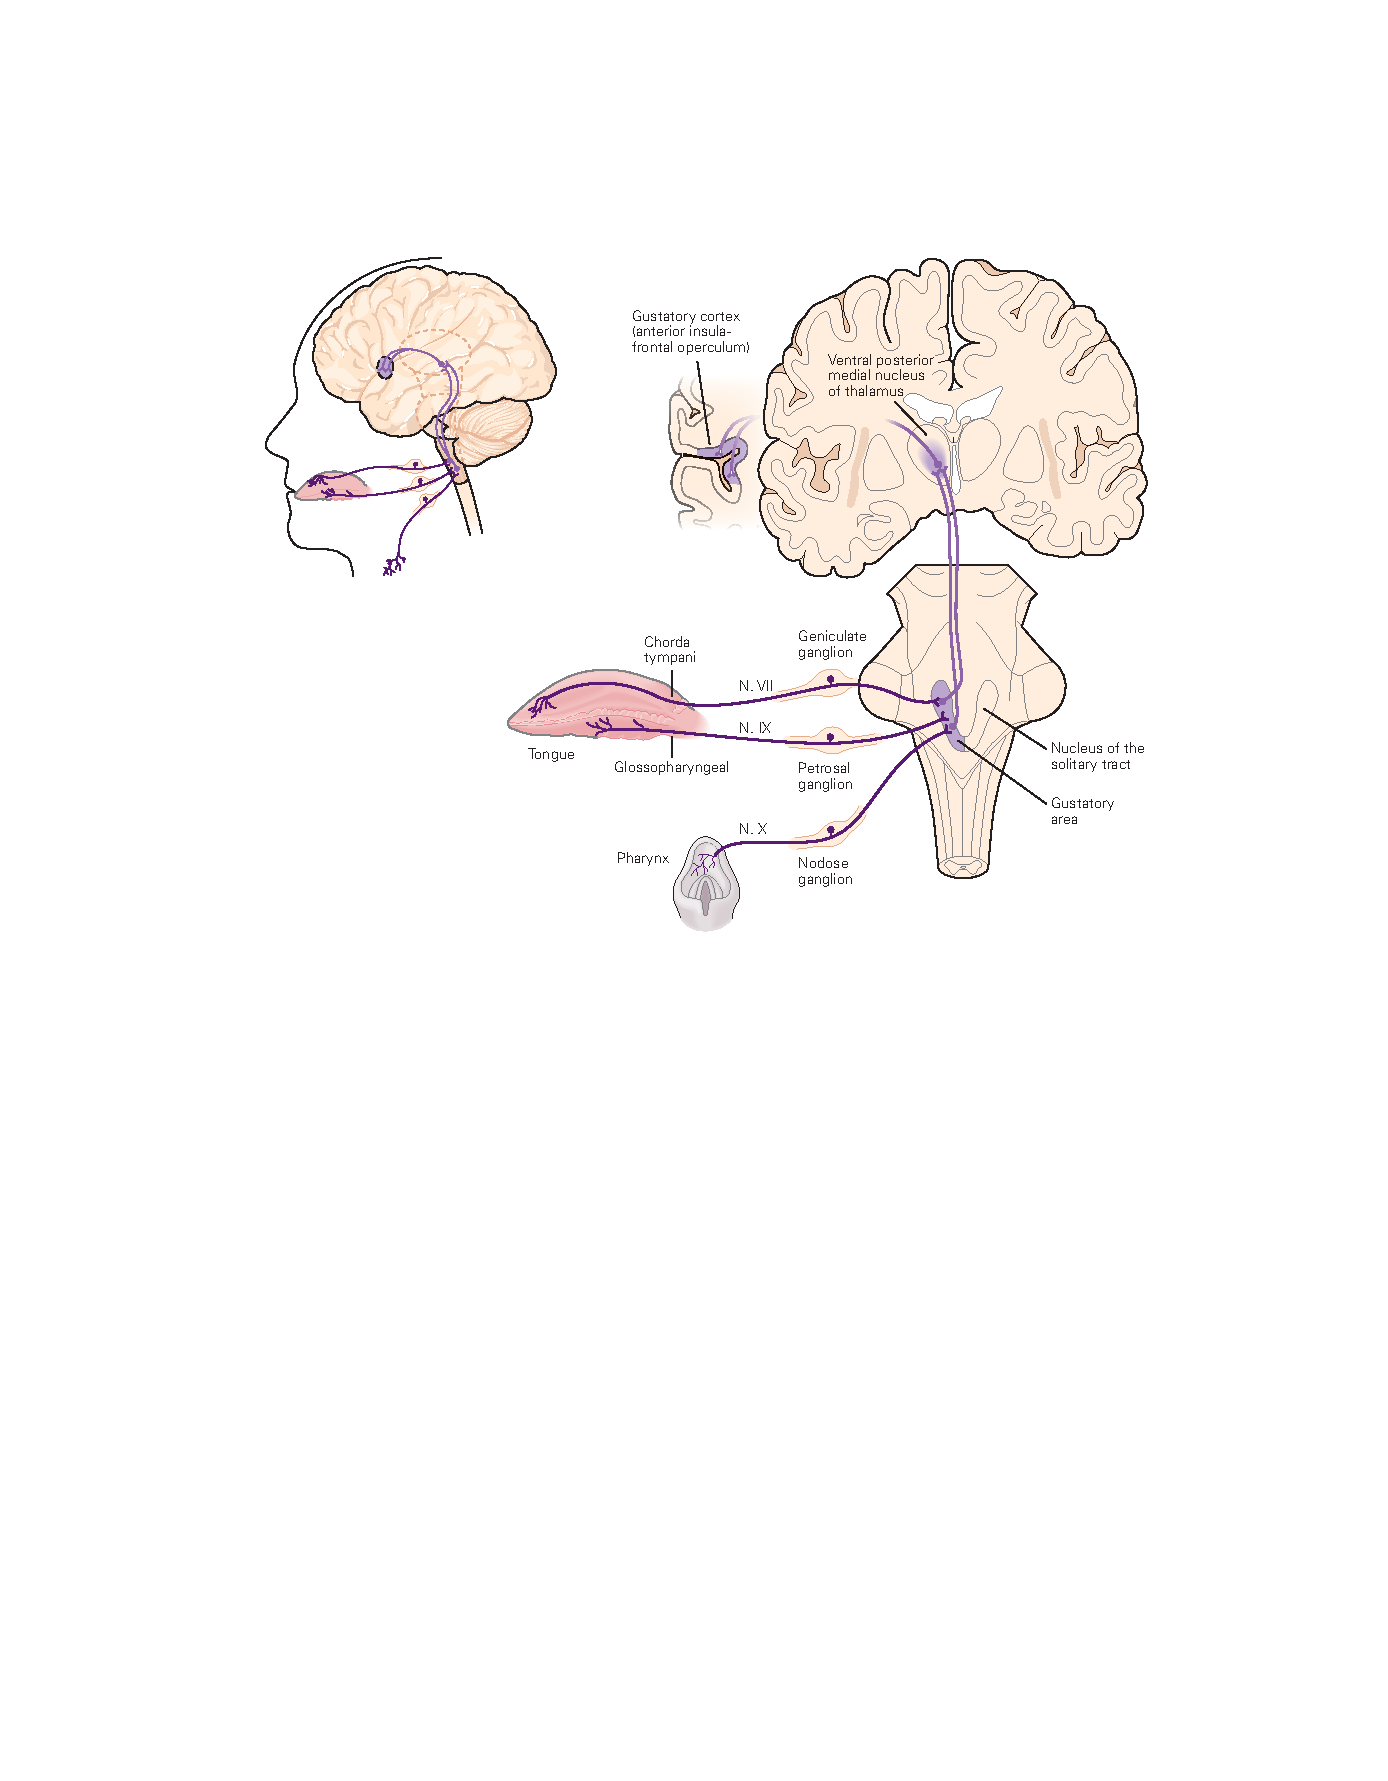
\includegraphics[width=0.8\linewidth]{chap29/fig_29_17}
	\caption{味觉系统。
		在口腔的味蕾中检测到促味剂。
		舌头和咽部的味蕾受味觉感觉神经元的外周纤维支配,这些神经元在舌咽神经、鼓索神经和迷走神经中行进,并终止于脑干孤束核。
		从那里,味觉信息通过丘脑传递到味觉皮层和下丘脑。}
	\label{fig:29_17}
\end{figure}



\subsection{每种味觉形态都由不同的感觉受体和细胞检测}

五种味觉品质由不同味觉细胞微绒毛中的感觉受体检测。 
有两种一般类型的受体:
苦味、甜味和鲜味促味剂与 G 蛋白偶联受体相互作用,而咸味和酸味促味剂直接与特定离子通道相互作用(图 ~\ref{fig:29_14})。 
这些相互作用使味觉细胞去极化,导致传入味觉纤维产生动作电位。


\begin{figure}[htbp]
	\centering
	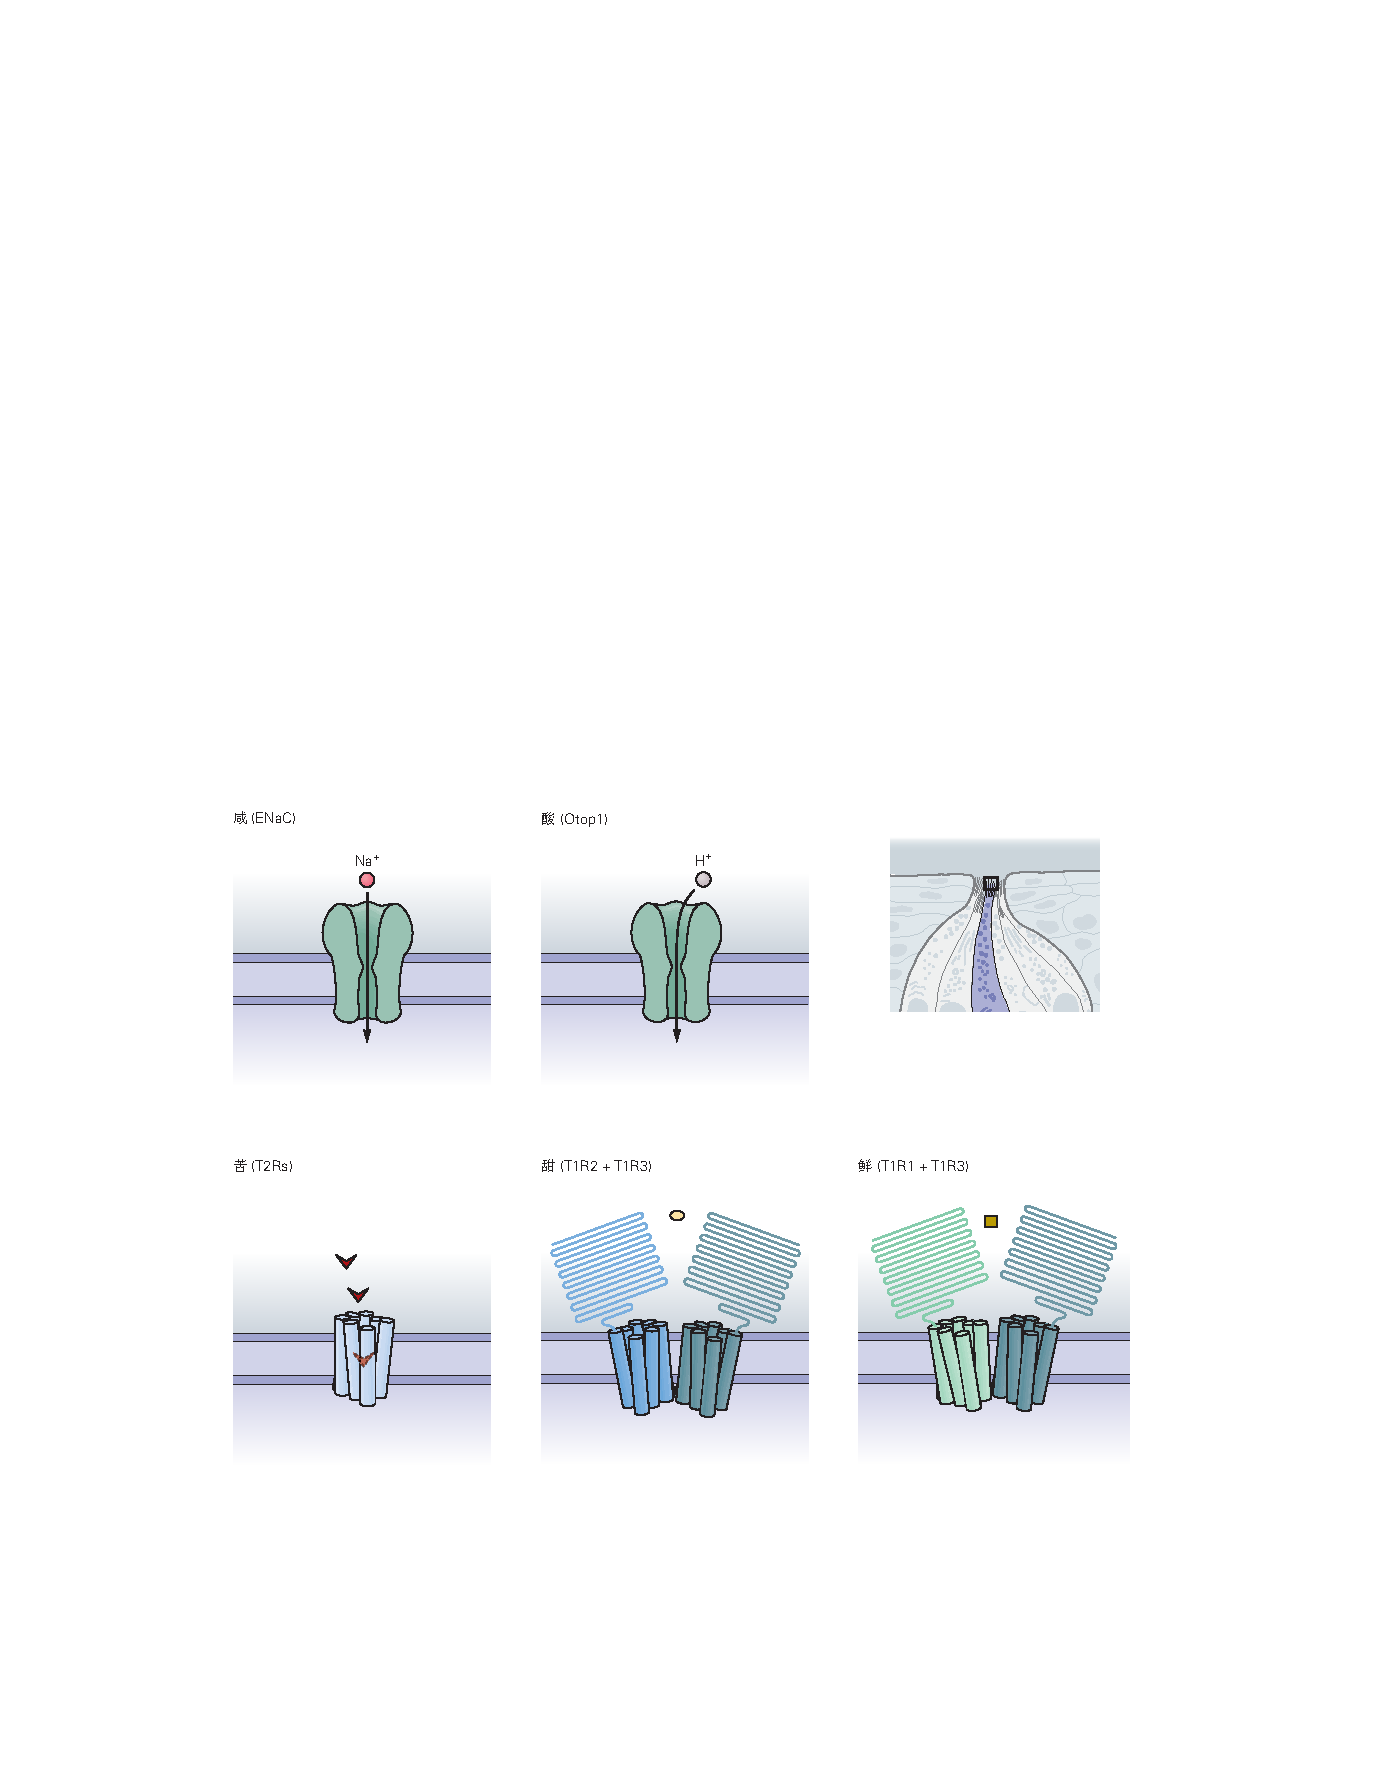
\includegraphics[width=0.75\linewidth]{chap29/fig_29_14}
	\caption{味觉细胞中的感觉转导。
		不同的味觉品质涉及味觉细胞顶端微绒毛的不同检测机制(见图 \ref{fig:29_13} B)。
		咸味和酸味促味剂直接激活离子通道,而被感知为苦味、甜味或鲜味的促味剂激活 G 蛋白偶联受体。 苦味元由 T2R 受体检测,而甜味元由 T1R2 和 T1R3 的组合检测,鲜味元由 T1R1 和 T1R3 的组合检测。}
	\label{fig:29_14}
\end{figure}


甜味受体

人类认为甜的化合物包括糖、人工甜味剂(如糖精和阿斯巴甜)、一些蛋白质(如莫内林和奇异果甜蛋白)以及几种 d-氨基酸。
所有这些甜味化合物均由异聚受体检测,该异聚受体由 T1R 味觉受体家族的两个成员 T1R2 和 T1R3 组成(图~\ref{fig:29_15})。
T1R 受体是一个由三个相关的 G 蛋白偶联受体组成的小家族,它们参与甜味和鲜味检测。


\begin{figure}[htbp]
	\centering
	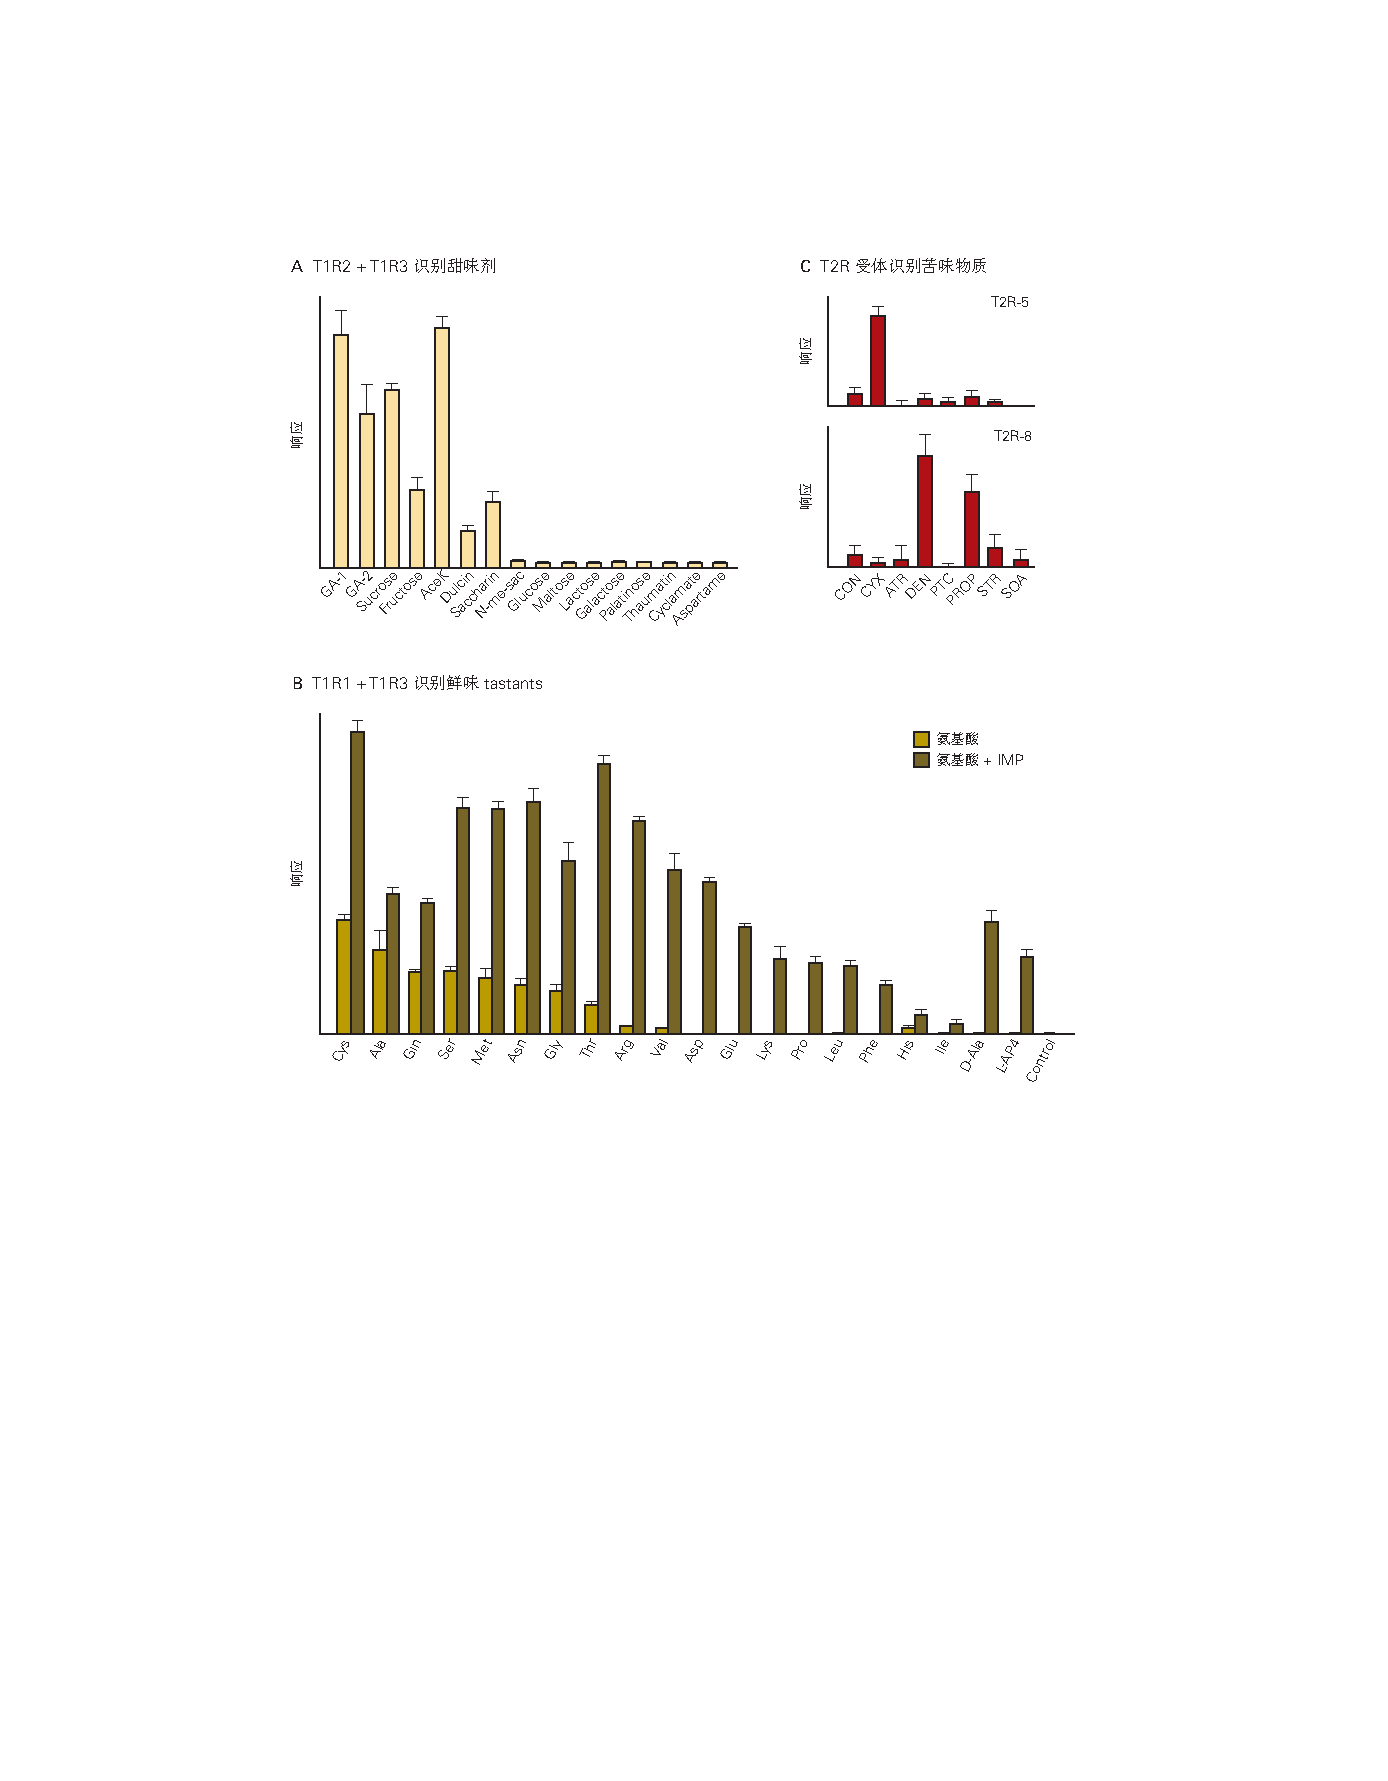
\includegraphics[width=0.8\linewidth]{chap29/fig_29_15}
	\caption{由 T1R 和 T2R 受体识别的促味剂。
		钙敏感性染料用于测试在组织培养细胞系中表达的 T1R 和 T2R 受体是否可以检测促味剂。
		\textbf{A.} 表达大鼠 T1R2 和大鼠 T1R3 的细胞对多种甜味化合物有反应。
		\textbf{B.} 表达小鼠 T1R1 和小鼠 T1R3 的细胞对多种 l-氨基酸(鲜味)有反应。
		肌苷一磷酸 (IMP) 可增强反应。
		\textbf{C.} 表达不同 T2R 受体的细胞选择性地响应不同的苦味化合物。
		表达小鼠 T2R5 的细胞对环己酰亚胺 (CYX) 反应最强烈,而表达小鼠 T2R8 的细胞优先对地那铵 (DEN) 和 6-正丙基-2-硫氧嘧啶 (PROP) 反应。
		(ATR,阿托品;CON,对照;PTC,苯基硫脲;SOA,蔗糖八乙酸酯;STR,士的宁。)}
	\label{fig:29_15}
\end{figure}


TIR 家族的受体有一个大的 N 末端细胞外结构域(图 ~\ref{fig:29_14}),它作为主要的配体结合结构域,类似于犁鼻神经元的 V2R 受体。
该结构域识别许多不同的糖,在毫摩尔范围内具有低亲和力结合。
这可确保仅检测到具有营养价值的高糖浓度。
改变小鼠这个区域的单个氨基酸可以改变动物对甜味化合物的敏感性。
事实上,T1R3 最初是通过检查小鼠糖精偏好 (Sac) 基因座的基因发现的,该基因座是控制对糖精、蔗糖和其他甜味化合物敏感性的染色体区域。


在小鼠中,具有 T1R2 受体的味觉细胞主要存在于上颚、叶状和周缘乳头中;
几乎无一例外,这些细胞也拥有 T1R3 受体(图 ~\ref{fig:29_16} A)。
小鼠基因敲除实验表明,T1R2/T1R3 复合物可介导除高浓度糖类以外的所有甜味化合物的检测,高浓度糖类也可单独由 T1R3 检测。


\begin{figure}[htbp]
	\centering
	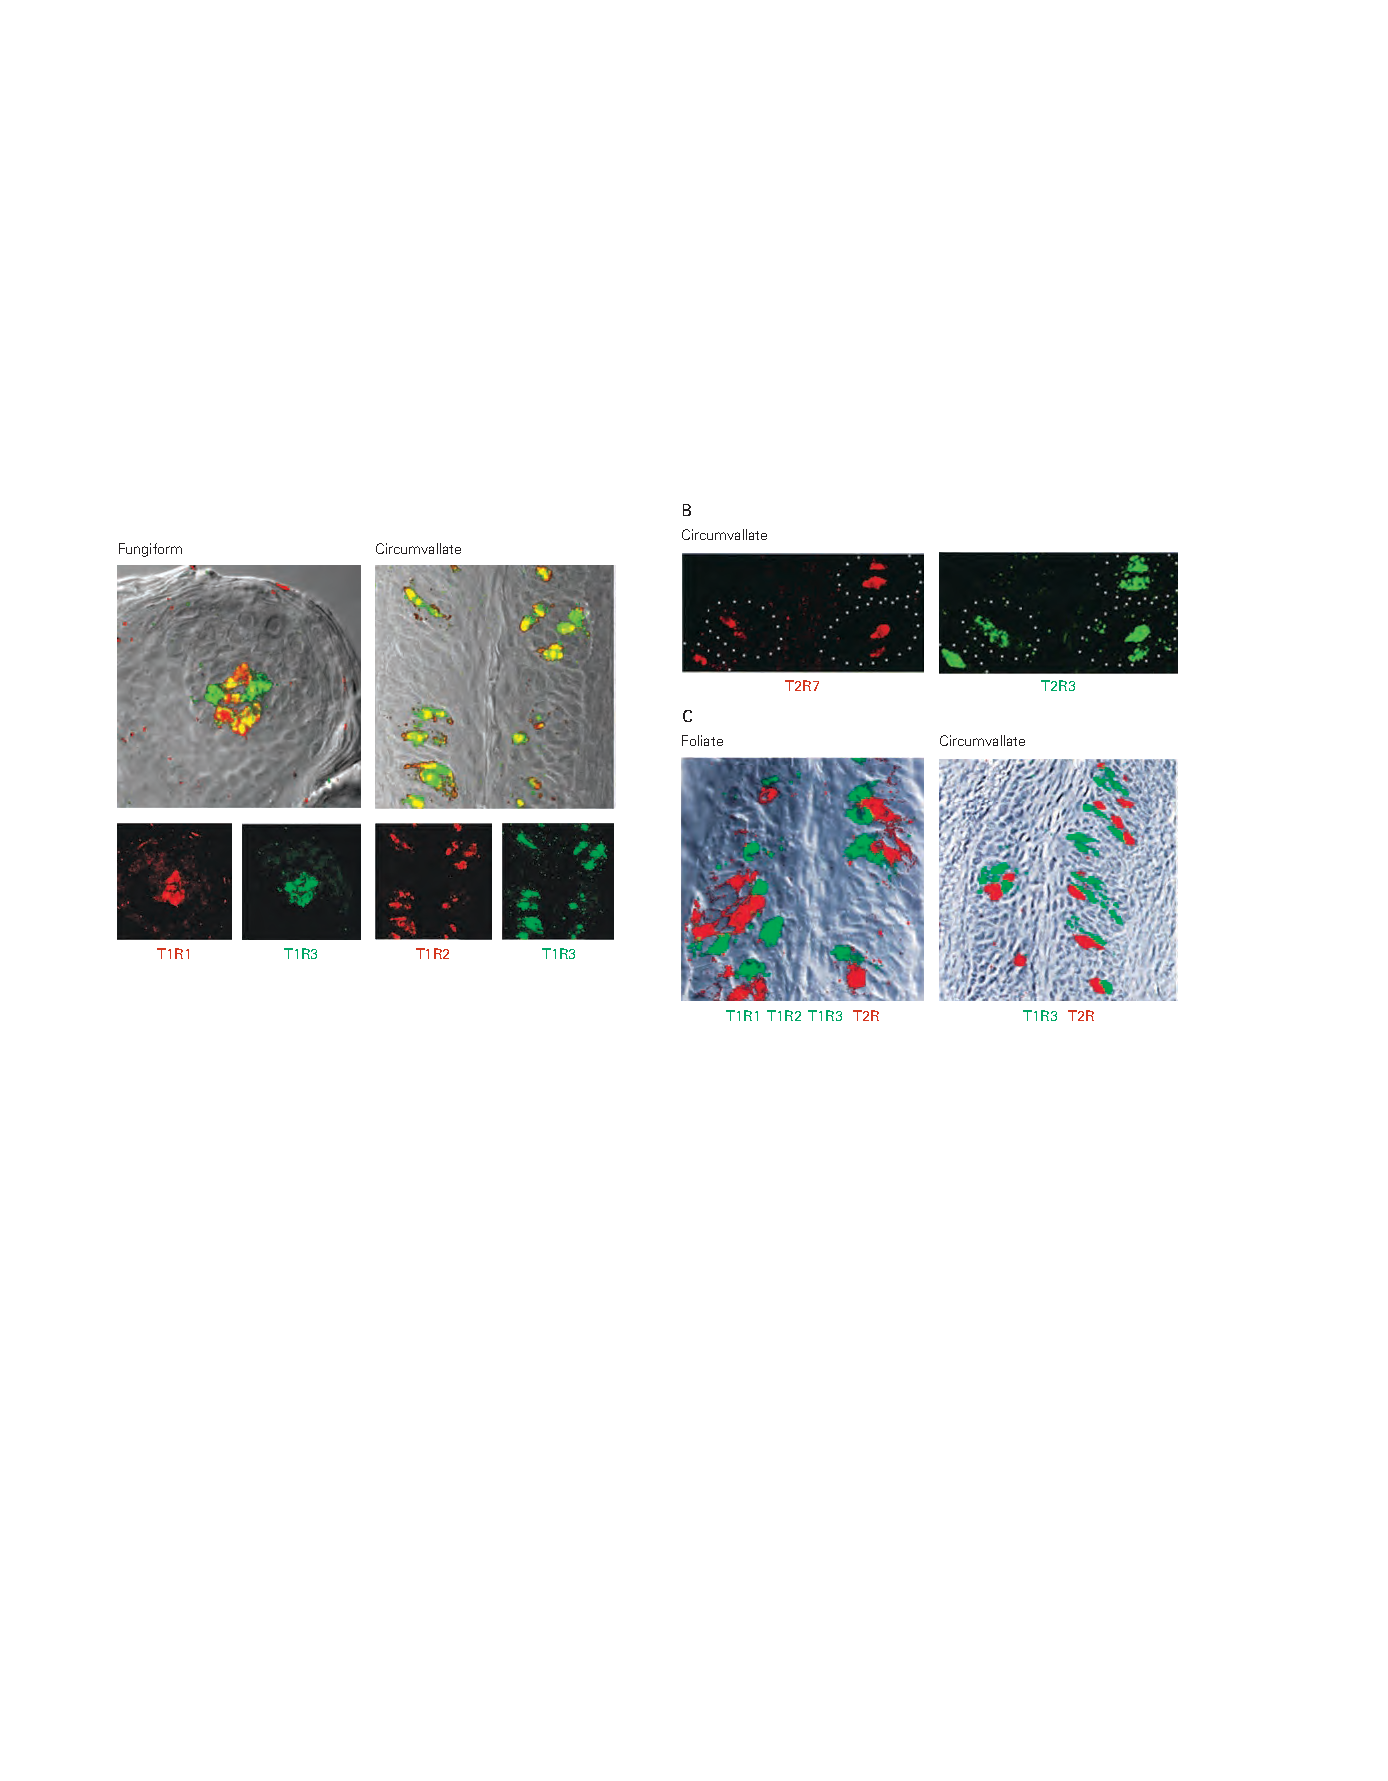
\includegraphics[width=0.5\linewidth]{chap29/fig_29_16}
	\caption{(右)T1R 和 T2R 受体在舌头上的表达。 小鼠或大鼠舌头的切片与标记 T1R 或 T2R \textit{信使核糖核酸}的探针杂交,以检测它们在味觉细胞中的表达位点。
		\textbf{A.} T1R3 受体在所有三种乳头的味觉细胞中均有表达。
		然而,T1R1 主要存在于菌状乳头中,而 T1R2 主要位于周缘(和叶状)乳头中。
		表达位点之间的重叠在顶部的显微照片中显示为黄色细胞。
		T1R1-T1R3 鲜味受体更常见于菌状乳突中,而 T1R2-T1R3 甜味受体更常见于环状乳突和叶状乳突中。
		\textbf{B.} 检测促苦味剂的味觉细胞可以表达 T2R 受体的多种变体。
		在这里,T2R3 和 T2R7 的探针标记了 circumvallate papillae 中的相同味觉细胞。
		\textbf{C.} T1R 和 T2R 受体在不同的味觉细胞中表达。
		由 T1R3 探针或混合 T1R 探针(绿色)标记的味觉细胞与由 T2R 探针混合物(红色)标记的细胞不重叠。}
	\label{fig:29_16}
\end{figure}


\textit{鲜味感受器}

鲜味是指谷氨酸钠的咸味,谷氨酸钠是一种广泛用作增味剂的氨基酸。
据信,与鲜味相关的愉悦感觉会促进蛋白质的摄入,因此在进化上对营养很重要。


鲜味受体是两个 T1R 受体亚基的复合物:T1R1,特异于鲜味受体,以及T1R3,存在于糖和鲜味受体中(图~\ref{fig:29_14})。
在小鼠中,T1R1/T1R3 复合物可以与所有 l-氨基酸相互作用(图~\ref{fig:29_15}B),但在人类中它优先被谷氨酸激活。
嘌呤核苷酸,如肌苷 5'-单磷酸 (IMP),通常被添加到谷氨酸钠中以增强其令人愉悦的鲜味。
有趣的是,体外研究表明,IMP 增强了 T1R1/T1R3 对 l-氨基酸的反应性,充当受体的强正变构调节剂(图~\ref{fig:29_15}B)。


具有 T1R1 和 T1R3 的味觉细胞集中在菌状乳头中(图~\ref{fig:29_16}A)。
对删除了单个 T1R 基因的基因工程小鼠进行的研究表明,T1R1/T1R3 复合物只负责鲜味,而 T1R2/T1R3 只负责甜味。
正如预期的那样,T1R1 的基因敲除选择性地消除了鲜味,T1R2 的基因敲除特异性地消除了甜味,而 T1R3 的基因敲除同时消除了甜味和鲜味(正如预测的那样,因为它是鲜味和鲜味的共同亚基) 甜味感受器)。


甜味和鲜味受体在不同物种之间存在显着差异。
最有趣的是,某些物种丢失了不同的 T1R 亚基,这可能反映了它们的进化生态位和饮食。
例如,几乎完全以竹子为食的大熊猫缺乏功能性的鲜味感受器。
另一方面,家猫、老虎和猎豹没有功能性甜味受体,而以血液为食的吸血蝙蝠则发生突变,消除了甜味和鲜味功能受体。



\textit{苦味受体}

苦味被认为是作为有毒分子的厌恶信号进化而来的。
苦味感是由多种化合物引起的,包括咖啡因、尼古丁、生物碱和地那铵,这是已知的最苦的化学物质(有时将这种化合物添加到无味无味的有毒产品中以防止其摄入)。


促苦味剂由大约 30 个称为 T2R 的 G 蛋白偶联受体家族检测(图~\ref{fig:29_14})。
然而,不同的动物物种含有不同数量的苦味受体(从鸡基因组中的少数到西方爪蛙中的 50 多个不等;
人类有 28 个 T2R 基因)。
这些受体识别具有不同化学结构的苦味化合物,调整每个 T2R 以检测少量苦味化合物(图~\ref{fig:29_15} C)。
T2R 受体识别在微摩尔范围内具有高亲和力结合的化学物质,从而可以检测微量的有害化合物。
单个味觉细胞表达许多(可能是大多数)类型的 T2R 受体(图~\ref{fig:29_16}B)。
这种排列意味着关于不同促苦味剂的信息被整合到各个味觉细胞中。
因为不同的苦味化合物被相同的细胞检测到,所以所有这些化合物都会引起相同的感知苦味质量。
苦味的程度可能是由化合物激活苦味细胞的有效性引起的。


有趣的是,已经在人类和老鼠身上发现了感知特定苦味化合物能力的遗传差异。
例如,对于苦味化学物质 6-正丙基硫氧嘧啶,人类要么是超级味觉者、品尝者,要么是味盲。
正是通过将这种性状的变异映射到特定的染色体位点,然后通过在该染色体区间内寻找新的 G 蛋白偶联受体基因,T2R 受体才被首次识别出来。
在检测 6-n-丙基硫氧嘧啶的情况下,导致遗传差异的基因已被证明是特定的 T2R 基因。
因此,一些苦味化合物可能主要被大约 30 种 T2R 受体类型中的一种识别。


表达 T2R 受体的味觉细胞存在于小鼠的叶状乳头和周缘乳头中(图~\ref{fig:29_16}C)。
给定的味觉细胞表达 T2R 或 T1R 受体(即一种味觉细胞 - 一种受体类别),但单个味蕾可以包含所有类型的味觉细胞(例如,甜味、鲜味、苦味)。
细胞的这种混合符合观察结果,即一个味蕾可以被不止一类促味剂激活; 例如,甜味和苦味。



\textit{咸味感受器}

盐的摄入对于维持电解质平衡至关重要。
也许是因为电解质必须保持在一个严格的范围内,对盐的行为反应是浓度依赖性的:低盐浓度是有食欲的,而高盐浓度是厌恶的。
对盐的反应如何根据浓度变化?
事实证明,多个味觉细胞可以检测盐分。
必需的盐味感受器细胞使用上皮钠通道 ENaC(见图~\ref{fig:29_14})。
这些专门的盐味受体不同于甜味、苦味或鲜味受体。
在高得多的盐浓度下,一些苦味和酸味细胞也会对盐产生反应,尽管检测的分子细节尚未确定。
因此,盐的食欲浓度通过盐敏感细胞中的 ENaC 盐味受体驱动反应,而高盐浓度会激活苦味和酸味细胞,从而引发行为厌恶。



\textit{酸味感受器}

酸味与酸性或发酵食品或饮料有关。
与苦味化合物一样,动物天生就厌恶酸味物质,这表明酸味的适应性优势是避免变质食物。
与其他 4 种味觉品质一样,酸味也由其自身类型的味觉感受器细胞检测到(图~\ref{fig:29_14})。
离子通道 Otopetrin-1 (Otop1) 是一种质子选择性通道,通常参与前庭系统的重力感觉,是味觉系统中的酸味离子通道。
正如预期的那样,小鼠中 Otop1 的敲除消除了酸味受体细胞对酸的反应。
此外,经改造在甜味受体细胞中表达 Otop1 的小鼠现在拥有对酸味刺激也有反应的甜味细胞,表明该通道足以赋予酸感。


分子遗传学研究表明,不同的味觉形态是由不同的味觉细胞亚群检测到的。
正如我们所见,T1R1 和 T1R3 的组合负责所有鲜味,所有甜味检测都需要 T1R2 和 T1R3 的组合,但高浓度糖的检测除外,这可以由 T1R3 单独介导。
T1R1 和 T1R2 受体由不同的味觉细胞亚群表达,表明甜味和鲜味促味剂的检测是分开的。
同样,受体和分子标记独特地定义了苦味、低盐味和酸味细胞。


对缺乏特定味觉受体基因或细胞类型的小鼠的研究表明,每种味觉品质都由不同类别的味觉细胞检测到。
这些研究表明,一种味觉形态的丧失不会影响其他味觉形态。
例如,甜味细胞已被基因切除的小鼠无法检测到糖分,但仍能检测到氨基酸、苦味化合物、盐和酸味化合物。
同样,被设计为缺乏特定味觉感受器的小鼠无法检测到相应的促味剂。
例如,缺乏选择性苦味受体的小鼠对相应的促苦味剂没有反应,而缺乏 ENaC 的小鼠则无法检测到盐的味道。
这些类型的研究表明,不同的味觉是由驱动特定行为的不同类别的味觉细胞中表达的不同受体检测到的。


对老鼠的研究进一步表明,决定动物对促味剂反应的是味觉细胞,而不是受体。
人类苦味受体 T2R16 识别小鼠无法检测到的促苦味剂。
当这种受体在通常表达 T2R 苦味受体的小鼠味觉细胞中表达时,配体会引起强烈的味觉厌恶。
然而,当该受体在表达 T1R2/T1R3 甜味复合物的细胞(即甜味细胞)中表达时,苦味配体会引发强烈的味觉接受。
这些发现表明,小鼠对不同促味剂(在本例中为甜味和苦味)的先天反应是通过标记线起作用的,这些标记线将不同味觉细胞亚群的激活与不同的行为结果联系起来。



\subsection{味觉信息从外围传递到味觉皮层}

每个味觉细胞的基部都由初级感觉神经元轴突的外围分支支配(图~\ref{fig:29_13})。
每条感觉纤维分支多次,支配味蕾内的多个味觉细胞。
神经递质从味觉细胞释放到感觉纤维上,在纤维中引起动作电位,并将信号传输到感觉细胞体。


味觉感觉神经元的细胞体位于膝状体、岩骨和结状神经节中。
这些神经元的外周分支在颅神经 VII、IX 和 X 中传播,而中央分支进入脑干,在那里它们终止于孤束核味觉区的神经元(图~\ref{fig:29_17})。
在大多数哺乳动物中,该核中的神经元将信号传递到脑桥的臂旁核,脑桥又将味觉信息传递到丘脑的腹后内侧核。 
然而,在灵长类动物中,这些神经元将味觉信息直接传递到丘脑的味觉区。


味觉信息从丘脑传输到味觉皮层,味觉皮层是位于前岛叶和额盖之间边界的大脑皮层区域(图~\ref{fig:29_17})。
味觉皮层被认为调节味觉刺激的有意识感知和辨别。
丘脑和皮层的味觉区也直接或间接地将信息传递给控制进食行为和自主反应的下丘脑。


大规模钙成像显示味觉皮层中的一些神经元优先响应一种味觉形态,例如苦味或甜味。
这些神经元位于隔离的皮层区域或热点中。
有趣的是,使用光激活离子通道激活甜蜜热点中的神经元会引发天生有吸引力的反应。
相比之下,苦味热点的激活会引起舔舐和强烈厌恶口面部反应的抑制,模仿常见的对促苦味剂的反应。
这些实验表明,直接控制初级味觉皮层可以唤起特定、可靠和稳健的行为,这些行为模仿对天然促味剂的反应。
他们还说明味觉通路可以激活对甜味和苦味化学物质的先天、即时反应。
为了证明这些皮层触发的行为是天生的(即,独立于学习或经验),在从未尝过甜味或苦味化学物质(突变消除了所有甜味和苦味信号转导)的突变小鼠中进行了类似的刺激实验。
即使在这些动物中,相应皮层区域的激活也触发了预期的行为反应,从而证实了味觉的预定性质。



\subsection{对味道的感知取决于味觉、嗅觉和体感输入}

我们所认为的食物风味的大部分来源于味觉和嗅觉系统整合所提供的信息。
伴随咀嚼和吞咽的舌头、脸颊和喉咙的运动将口腔中食物或饮料释放的挥发性分子泵入鼻腔后部(“鼻后通道”)。 
尽管鼻子的\textit{嗅上皮}明显对味觉有重要贡献,但这种感觉局限于口腔而不是鼻子。


体感系统也被认为参与了这种风味定位。
味觉、舌头的体感刺激和气味物质通过鼻后通道进入鼻子之间的重合被认为导致气味物质在口中被感知为味道。
味道的感觉也经常有体感成分,包括食物的质地以及辛辣或薄荷食物和碳酸化引起的感觉。



\subsection{昆虫具有驱动先天行为的特定形态的味觉细胞}

昆虫有专门的味觉系统,可以评估食物中的潜在营养素和毒素。
在长鼻、内部口器、腿、翅膀和产卵器上发现了味觉神经元,使昆虫能够在摄入前对当地的化学环境进行采样。
与哺乳动物一样,只有几种不同类型的味觉细胞能检测到不同的味道。
在果蝇中,不同的味觉细胞类别包括那些感知糖、苦味化合物、水和信息素的细胞。
与哺乳动物一样,这些不同味觉细胞的激活会驱动不同的先天行为;
例如,糖细胞的激活驱动食物接受行为,而苦味细胞的激活驱动食物排斥。
因此,尽管进化历史不同,但昆虫和哺乳动物味觉检测的基本组织非常相似。


昆虫的味觉感受器与脊椎动物的味觉感受器无关。
\textit{味觉感受器}基因家族的成员参与糖和苦味化合物的检测。
\textit{味觉感受器}是与苍蝇的气味受体远相关的跨膜受体。
苍蝇有大约 70 个\textit{味觉感受器}基因,考虑到它有大约 60 个嗅觉受体基因,这个数字多得惊人。
在糖细胞和苦味细胞中发现了不同的\textit{味觉感受器},许多\textit{味觉感受器}存在于单个神经元中。
除了遗传资源外,其他基因家族也参与昆虫味觉,包括离子型谷氨酸受体和其他离子通道类别的变体。
与嗅觉检测类似,参与味觉识别的基因家族在不同门类中存在差异,这表明用于化学识别的基因家族是独立进化的。



\section{要点}

1. 鼻子中的气味检测是由一大类气味受体介导的,人类大约有 350 个,小鼠大约有 1 千个。
这些受体的蛋白质序列各不相同,这与检测结构多样的气味剂的能力一致。


2. 单个气味受体可以检测多种气味,不同的气味激活不同的受体组合。
这种组合策略解释了我们如何区分多种气味剂以及几乎相同的气味剂如何具有不同的气味。


3. 鼻子中的每个嗅觉感觉神经元都表达一种类型的受体。
数以千计具有相同受体的神经元分散在\textit{嗅上皮}细胞中,并与表达其他受体的神经元混合在一起。


4. 在嗅球中,表达相同受体的感觉神经元的轴突会聚在一些受体特异性肾小球中,生成个体间相似的气味受体输入图。


5. 嗅球投射神经元的轴突广泛投射到嗅觉皮层的多个区域,产生高度分布的皮层神经元组织,对个别气味有反应。
嗅觉皮层将信息传输到许多其他大脑区域。


6. 在老鼠身上,可以在鼻子或犁鼻器中检测到信息素,这是人类所没有的结构。
来自鼻子和犁鼻器的信号通过大脑中的不同神经通路传播。


7. 果蝇 Drosophila melanogaster 的嗅觉系统在许多方面类似于哺乳动物。
它使用大量不同的嗅觉受体,每个嗅觉感觉神经元表达一个或几个嗅觉受体。
此外,在大脑触角叶的一些特定肾小球中,具有相同受体突触的神经元。
从那里,嗅觉信号被传输到两个主要的大脑区域,这些区域涉及先天和习得的气味反应。
在果蝇中使用遗传方法的简便性使得能够快速研究气味编码和行为的机制。


8. 味觉系统检测五种基本味道:甜、酸、苦、咸和鲜味(氨基酸)。
激活这些味觉品质的促味剂被主要位于舌头和上颚上皮味蕾中的味觉受体细胞检测到。
五种不同味觉形态的检测由不同的味觉感受器细胞介导,每个感受器细胞专用于一种形态。


9. 甜味元由单一类型的受体检测,该受体由两个亚基 T1R2 和 T1R3 组成。
鲜味受体是相关的,但包含 T1R1 和 T1R3 亚基的组合。


10. 苦味受体由大约 30 种相关但不同的受体组成,配体特异性各不相同。
单个味觉受体细胞表达许多或所有苦味受体。 


11. 与甜味、鲜味和苦味受体(它们都是 G 蛋白偶联受体)相比,咸味和酸味通过离子通道检测:ENaC 检测盐味,Otopetrin-1 检测酸味。 


12. 味觉信号从味蕾通过颅神经从膝状体、岩骨和结状神经节中的味觉感觉神经元通过标记线(甜味受体细胞到甜味神经元,苦味细胞到苦味神经元等)传播。
然后它们到达孤束核和臂旁核的味觉区,然后从那里到达丘脑的味觉区,然后到达味觉皮层。
反过来,味觉皮层投射到许多大脑区域,包括那些涉及运动控制、进食、享乐价值、学习和记忆的区域。


13. 味觉皮层包含甜味和苦味的热点,当直接受到刺激时,可以引发类似于将促味剂应用于舌头所获得的行为反应。 


14. 果蝇 Drosophila 也有专门的味觉系统,可以评估食物中的潜在营养素和毒素。
不同类别的味觉细胞感知糖、苦味化合物、信息素或水。 
这些不同的外围传感器的激活会驱动不同的先天行为,例如接受或拒绝食物。


